\documentclass[10pt]{article} 
\usepackage{amsmath}
\usepackage{listings}
\usepackage{hyperref}
\usepackage{fancyhdr}
\usepackage{graphicx}
\usepackage{tabularx}
\usepackage{color}
\usepackage{alltt}
\usepackage{rotating}
\usepackage{xtab}
\usepackage{calc}
\usepackage{appendix}
\usepackage{subfigure}

\hbadness=10000 % No "underfull hbox" messages

\begin{document}

%\lstset{language=C}

% Define the OpenFlow version here
\newcommand{\ofversion}{1.1.0}

% Calculations of widths for multipage tables
%
% Action table
\newlength{\atactionwidth}
\newlength{\atassocwidth}
\newlength{\atdescwidth}
\setlength{\atactionwidth}{0.25\textwidth - 2 \tabcolsep}
\setlength{\atassocwidth}{0.30\textwidth - 2 \tabcolsep}
\setlength{\atdescwidth}{0.45\textwidth - 2 \tabcolsep}

\pagestyle{fancy}
\fancyhead{}
\lhead{OpenFlow Switch Specification}
\rhead{Version \ofversion}
\renewcommand{\headrulewidth}{0.4pt}
\renewcommand{\footrulewidth}{0.4pt}

\fontfamily{cmr} % what about cmss?
\selectfont

\title{OpenFlow Switch Specification}
\author{Version \ofversion{} ( Wire Protocol \input{define/OFP_VERSION})}
\date{\today}
\maketitle

\tableofcontents
\listoftables
\listoffigures
\clearpage

\section{Introduction}
This document describes the requirements of an OpenFlow Switch.  We recommend that you read the latest version of the OpenFlow whitepaper before reading this specification. The whitepaper is available on the  OpenFlow Consortium website (\url{http://openflow.org}). This specification covers the components and the basic functions of the switch, and the OpenFlow protocol to manage an OpenFlow switch from a remote controller.
\\\\

\begin{figure}[htbp]
\centering
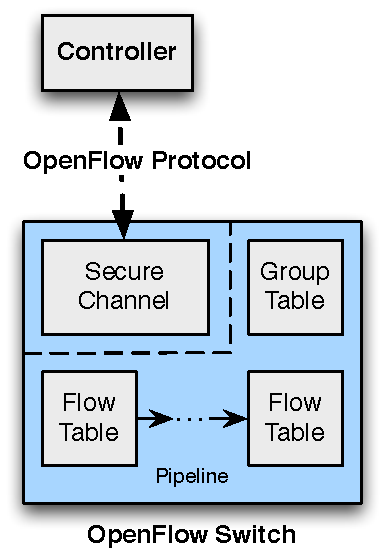
\includegraphics[height=2.8in]{switch_overview}
\caption{An OpenFlow switch communicates with a controller over a secure connection using the OpenFlow protocol.}
\label{fig:flow table and controller}
\end{figure}

\section{Switch Components}
An OpenFlow Switch consists of one or more \emph{flow tables} and a \emph{group table}, which perform packet lookups and forwarding, and an \emph{OpenFlow channel} to an external controller (Figure \ref{fig:flow table and controller}).  The controller manages the switch via the OpenFlow protocol.   Using this protocol, the controller can add, update, and delete \emph{flow entries}, both reactively (in response to packets) and proactively.
\\\\
Each flow table in the switch contains a set of flow entries; each flow entry consists of \emph{match fields}, \emph{counters}, and a set of \emph{instructions} to apply to matching packets (see \ref{ft:flowtableentry}).
\\\\
Matching starts at the first flow table and may continue to additional flow tables (see \ref{sec:pipeline}). Flow entries match packets in priority order, with the first matching entry in each table being used (see \ref{sec:matching}). If a matching entry is found, the instructions associated with the specific flow entry are executed. If no match is found in a flow table, the outcome depends on switch configuration: the packet may be forwarded to the controller over the OpenFlow channel, dropped, or may continue to the next flow table (see \ref{sec:pipeline}).
\\\\
Instructions associated with each flow entry describe packet forwarding, packet modification, group table processing, and pipeline processing (see \ref{ft:instructions}). Pipeline processing instructions allow packets to be sent to subsequent tables for further processing and allow information, in the form of metadata, to be communicated between tables. Table pipeline processing stops when the instruction set associated with a matching flow entry does not specify a next table; at this point the packet is usually modified and forwarded (see \ref{ft:actionset}).
\\\\
Flow entries may forward to a \emph{port}. This is usually a physical port, but it may also be a virtual port defined by the switch or a reserved virtual port defined by this specification. Reserved virtual ports may specify generic forwarding actions such as sending to the controller, flooding, or forwarding using non-OpenFlow methods, such as ``normal'' switch processing (see \ref{ft:actions}), while switch-defined virtual ports may specify link aggregation groups, tunnels or loopback interfaces (see \ref{ft:actions}).
\\\\
Flow entries may also point to a group, which specifies additional processing (see \ref{sec:group table}). Groups represent sets of actions for flooding, as well as more complex forwarding semantics (e.g. multipath, fast reroute, and link aggregation).  As a general layer of indirection, groups also enable multiple flows to forward to a single identifier (e.g. IP forwarding to a common next hop).  This abstraction allows common output actions across flows to be changed efficiently.
\\\\
The group table contains group entries; each group entry contains a list of \emph{action buckets} with specific semantics dependent on group type (see \ref{sec:group types}). The actions in one or more action buckets are applied to packets sent to the group.
\\\\
Switch designers are free to implement the internals in any way convenient, provided that correct match and instruction semantics are preserved. For example, while a flow may use an all group to forward to multiple ports, a switch designer may choose to implement this as a single bitmask within the hardware forwarding table.  Another example is matching; the pipeline exposed by an OpenFlow switch may be physically implemented with a different number of hardware tables.

\section{Glossary}
\label{sec:glossary}
This section describes key OpenFlow specification terms:
\begin{itemize}
\item \textbf{Byte}: an 8-bit octet.
\item \textbf{Packet}: an Ethernet frame, including header and payload.
\item \textbf{Pipeline}: the set of linked tables that provide matching, forwarding, and packet modifications in an OpenFlow switch.
\item \textbf{Port}: where packets enter and exit the OpenFlow pipeline. May be a physical port, a virtual port defined by the switch, or a virtual port defined by the OpenFlow protocol. Reserved virtual ports are ports reserved by this specification (see \ref{ft:actions}). Switch-defined virtual ports are higher level abstractions that may be defined in the switch using non-OpenFlow methods (e.g. link aggregation groups, tunnels, loopback interfaces).
\item \textbf{Match Field}: a field against which a packet is matched, including packet headers, the ingress port, and the metadata value.
\item \textbf{Metadata}: a maskable register value that is used to carry information from one table to the next.
\item \textbf{Instruction}: an operation that either contains a \emph{set} of actions to add to the action set, contains a \emph{list} of actions to apply immediately to the packet, or modifies pipeline processing.
\item \textbf{Action}: an operation that forwards the packet to a port or modifies the packet, such as decrementing the TTL field. Actions may be specified as part of the instruction set associated with a flow entry or in an action bucket associated with a group entry.
\item \textbf{Action Set}: a set of actions associated with the packet that are accumulated while the packet is processed by each table and that are executed when the instruction set instructs the packet to exit the processing pipeline.
\item \textbf{Group}: a list of action buckets and some means of choosing one or more of those buckets to apply on a per-packet basis.
\item \textbf{Action Bucket}: a set of actions and associated parameters, defined for groups.
\item \textbf{Tag}: a header that can be inserted or removed from a packet via push and pop actions.
\item \textbf{Outermost Tag}: the tag that appears closest to the beginning of a packet.
\end{itemize}

\section{OpenFlow Tables}
This section describes the components of flow tables and group tables, along with the mechanics of matching and action handling.

\subsection{Flow Table}
\label{ft:flowtableentry}

A flow table consists of flow entries.

\begin{table}[hbp]
\centering
\begin{tabular}{|c|c|c|}
\hline	
Match Fields & Counters & Instructions\\ 
\hline	
\end{tabular}
\caption{Main components of a flow entry in a flow table.}
\label{table:flow entry}
\end{table}

Each flow table entry (see Table \ref{table:flow entry}) contains: 
\begin{itemize} 
\item \textbf{match fields}: to match against packets. These consist of the ingress port and packet headers, and optionally metadata specified by a previous table.
\item \textbf{counters}: to update for matching packets
\item \textbf{instructions} to modify the action set or pipeline processing
\end{itemize} 

\subsubsection{Pipeline Processing}
\label{sec:pipeline}

\begin{figure}[htbp]
\centering
\subfigure[Packets are matched against multiple tables in the pipeline]{
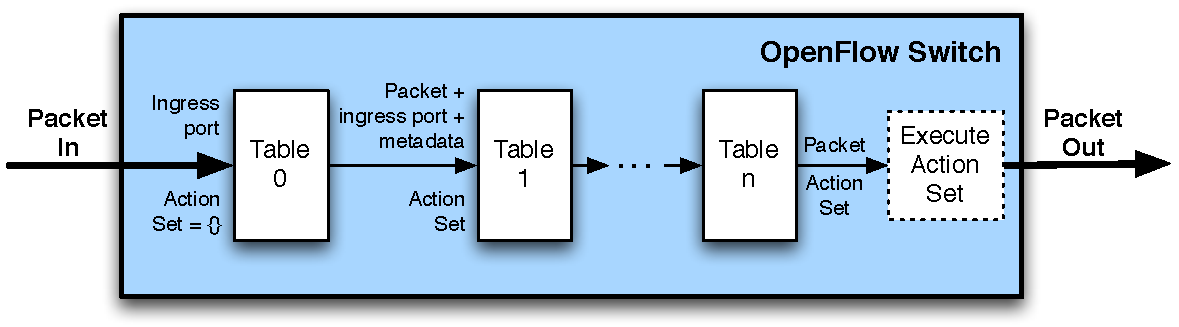
\includegraphics[width=\textwidth]{pipeline_flow_overview}
}
\subfigure[Per-table packet processing]{
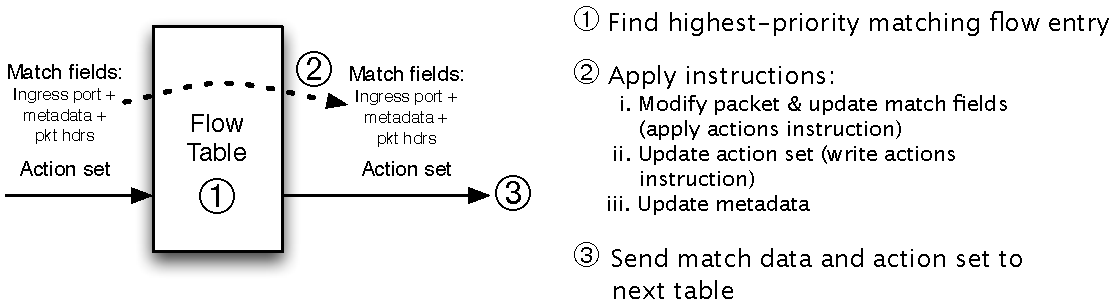
\includegraphics[width=\textwidth]{pipeline_flow_detail}
}
\caption{Packet flow through the processing pipeline}
\label{fig:packet flow multiple tables}
\end{figure}

OpenFlow-compliant switches come in two types: \emph{OpenFlow-only}, and \emph{OpenFlow-hybrid}. \textbf{OpenFlow-only} switches support only OpenFlow operation, in those switches all packets are processed by the OpenFlow pipeline, and can not be processed otherwise.
\\\\
\textbf{OpenFlow-hybrid} switches support both OpenFlow operation and \emph{normal} Ethernet switching operation, i.e. traditional L2 Ethernet switching, VLAN isolation, L3 routing, ACL and QoS processing. Those switches should provide a classification mechanism outside of OpenFlow that routes traffic to \emph{either} the OpenFlow pipeline or the normal pipeline. For example, a switch may use the VLAN tag or input port of the packet to decide whether to process the packet using one pipeline or the other, or it may direct all packets to the OpenFlow pipeline. This classification mechanism is outside the scope of this specification. An OpenFlow-hybrid switches may also allow a packet to go from the OpenFlow pipeline to the normal pipeline through the \emph{NORMAL} and \emph{FLOOD} virtual ports (see \ref{ft:actions}).
\\\\
The \textbf{OpenFlow pipeline} of every OpenFlow switch contains multiple flow tables, each flow table containing multiple flow entries. The OpenFlow pipeline processing defines how packets interact with those flow tables (see Figure \ref{fig:packet flow multiple tables}). An OpenFlow switch with only a single flow table is valid, in this case pipeline processing is greatly simplified.
\\\\
The flow tables of an OpenFlow switch are sequentially numbered, starting at 0. Pipeline processing always starts at the first flow table: the packet is first matched against entries of flow table 0. Other flow tables may be used depending on the outcome of the match in the first table.
\\\\
If the packet matches a flow entry in a flow table, the corresponding instruction set is executed (see \ref{sec:matching}). The instructions in the flow entry may explicitly direct the packet to another flow table (using the Goto Instruction, see \ref{ft:instructions}), where the same process is repeated again. A flow entry can only direct a packet to a flow table number which is greater than its own flow table number, in other words pipeline processing can only go forward and not backward. Obviously, the flow entries of the last table of the pipeline can not include the Goto instruction. If the matching flow entry does not direct packets to another flow table, pipeline processing stops at this table. When pipeline processing stops, the packet is processed with its associated action set and usually forwarded (see \ref{ft:actionset}).
\\\\
If the packet does not match a flow entry in a flow table, this is a table miss. The behavior on table miss depends on the table configuration; the default is to send packets to the controller over the control channel via a packet-in message (see \ref{sec:asynchronous}), another options is to drop the packet. A table can also specify that on a table miss the packet processing should continue; in this case the packet is processed by the next sequentially numbered table.

\subsection{Group Table}
\label{sec:group table}
A group table consists of group entries.  The ability for a flow to point to a \emph{group} enables OpenFlow to represent additional methods of forwarding (e.g. select and all).
\\\\
\begin{table}[hbp]
\centering
\begin{tabular}{|c|c|c|c|}
\hline
Group Identifier & Group Type & Counters & Action Buckets\\
\hline
\end{tabular}
\caption{A group entry consists of a group identifier, a group type, counters, and a list of action buckets.}
\label{table:group entry}
\end{table}
Each group entry (see Table \ref{table:group entry}) contains:
\begin{itemize}
\item \textbf{group identifier}: a 32 bit unsigned integer uniquely identifying the group
\item \textbf{group type}: to determine group semantics (see Section~\ref{sec:group types})
\item \textbf{counters}: updated when packets are processed by a group
\item \textbf{action buckets}: an ordered list of action buckets, where each action bucket contains a set of actions to execute and associated parameters
\end{itemize}

\subsubsection{Group Types}
\label{sec:group types}
The following group types are defined:

\begin{itemize}
\item \textbf{all}: Execute all buckets in the group.  This group is used for multicast or broadcast forwarding.  The packet is effectively cloned for each bucket; one packet is processed for each bucket of the group.  If a bucket directs a packet explicitly out the ingress port, this packet clone is dropped.  If the controller writer wants to forward out the ingress port, the group should include an extra bucket which includes a set-output-port action to the \verb|OFPP_IN_PORT| virtual port.
\item \textbf{select}: Execute one bucket in the group.  Packets are sent to a single bucket in the group, based on a switch-computed selection algorithm (e.g. hash on some user-configured tuple or simple round robin).  All configuration and state for the selection algorithm is external to OpenFlow.  When a port specified in a bucket in a select group goes down, the switch may restrict bucket selection to the remaining set (those with forwarding actions to live ports) instead of dropping packets destined to that port. This behavior may reduce the disruption of a downed link or switch.
\item \textbf{indirect}: Execute the one defined bucket in this group.  Allows multiple flows or groups to point to a common group identifier, supporting faster, more efficient convergence (e.g. next hops for IP forwarding).  This group type is effectively identical to an all group with one bucket.
\item \textbf{fast failover}: Execute the first live bucket.  Each action bucket is associated with a specific port and/or group that controls its liveness.  Enables the switch to change forwarding without requiring a round trip to the controller.  If no buckets are live, packets are dropped. This group type must implement a \textit{liveness mechanism}(see \ref{group_table:sec_chan:group_mod}).
\end{itemize}

\subsection{Match Fields}
\begin{table}[hbp]
\centering
\footnotesize
\begin{tabularx}{\textwidth}{ |X|X|X|X|X|X|X|X|X|X|X|X|X|XX|XX| }
\hline
\begin{sideways}Ingress Port \end{sideways} &
\begin{sideways}Metadata \end{sideways} &
\begin{sideways}Ether src \end{sideways} &
\begin{sideways}Ether dst \end{sideways} &
\begin{sideways}Ether type \end{sideways} &
\begin{sideways}VLAN id \end{sideways} &
\begin{sideways}VLAN priority \end{sideways} &
\begin{sideways}MPLS label \end{sideways} &
\begin{sideways}MPLS traffic class \end{sideways} &
\begin{sideways}IPv4 src \end{sideways} &
\begin{sideways}IPv4 dst \end{sideways} &
\begin{sideways}IPv4 proto / ARP opcode \end{sideways} &
\begin{sideways}IPv4 ToS bits \end{sideways} &
\begin{sideways}TCP/ UDP / SCTP src port \end{sideways} &
\begin{sideways}ICMP Type \end{sideways} &
\begin{sideways}TCP/ UDP / SCTP dst port \end{sideways} &
\begin{sideways}ICMP Code \end{sideways}
\\ 
\hline
\end{tabularx}
\caption{Fields from packets used to match against flow entries.}
\label{table:match fields}
\end{table}

Table \ref{table:match fields} shows the match fields an incoming packet is compared against. Each entry contains a specific value, or ANY, which matches any value. If the switch supports arbitrary bitmasks on the Ethernet source and/or destinations fields, or on the IP source and/or destination fields, these masks can more precisely specify matches.  The fields in the OpenFlow tuple are listed in Table \ref{table:match fields} and details on the properties of each field are described in Table \ref{table:header field details}. In addition to packet headers, matches can also be performed against the ingress port and metadata fields. Metadata may be used to pass information between tables in a switch.
\\\\
\begin{table}[hbp]
\centering
\footnotesize
\begin{tabularx}{\textwidth}{ |X|c|X|X| }
\hline Field & Bits & When applicable & Notes \\
\hline Ingress Port & 32 & All packets & Numerical representation of incoming port, starting at 1. This may be a physical or switch-defined virtual port. \\
\hline Metadata & 64 & Table 1 and above & \\
\hline Ethernet source address & 48 & All packets on enabled ports & Can use arbitrary bitmask \\
\hline Ethernet destination address & 48 & All packets on enabled ports & Can use arbitrary bitmask \\
\hline Ethernet type & 16 & All packets on enabled ports & An OpenFlow switch is required to match the type in both standard Ethernet and 802.2 with a SNAP header and OUI of 0x000000.  The special value of 0x05FF is used to match all 802.3 packets without SNAP headers. \\
\hline VLAN id & 12 & All packets with VLAN tags & VLAN identifier of \emph{outermost} VLAN tag. \\
\hline VLAN priority & 3 & All packets with VLAN tags & VLAN PCP field of \emph{outermost} VLAN tag. \\
\hline MPLS label & 20 & All packets with MPLS tags & Match on \emph{outermost} MPLS tag. \\
\hline MPLS traffic class & 3 & All packets with MPLS tags & Match on \emph{outermost} MPLS tag. \\
\hline IPv4 source address & 32 & All IPv4 and ARP packets & Can use subnet mask or arbitrary bitmask \\
\hline IPv4 destination address & 32 & All IPv4 and ARP packets & Can use subnet mask or arbitrary bitmask \\
\hline IPv4 protocol / ARP opcode & 8 & All IPv4 and IPv4 over Ethernet, ARP packets & Only the lower 8 bits of the ARP opcode are used \\
\hline IPv4 ToS bits & 6 & All IPv4 packets & Specify as 8-bit value and place ToS in upper 6 bits. \\
\hline Transport source port / ICMP Type & 16 & All TCP, UDP, SCTP, and ICMP packets & Only lower 8 bits used for ICMP Type \\
\hline Transport destination port / ICMP Code & 16 & All TCP, UDP, SCTP, and ICMP packets & Only lower 8 bits used for ICMP Code \\
\hline
\end{tabularx}
\caption{Field lengths and the way they must be applied to flow entries.}
\label{table:header field details}
\end{table}

\subsection{Matching}
\label{sec:matching}
\begin{figure}[!htb]
\centering
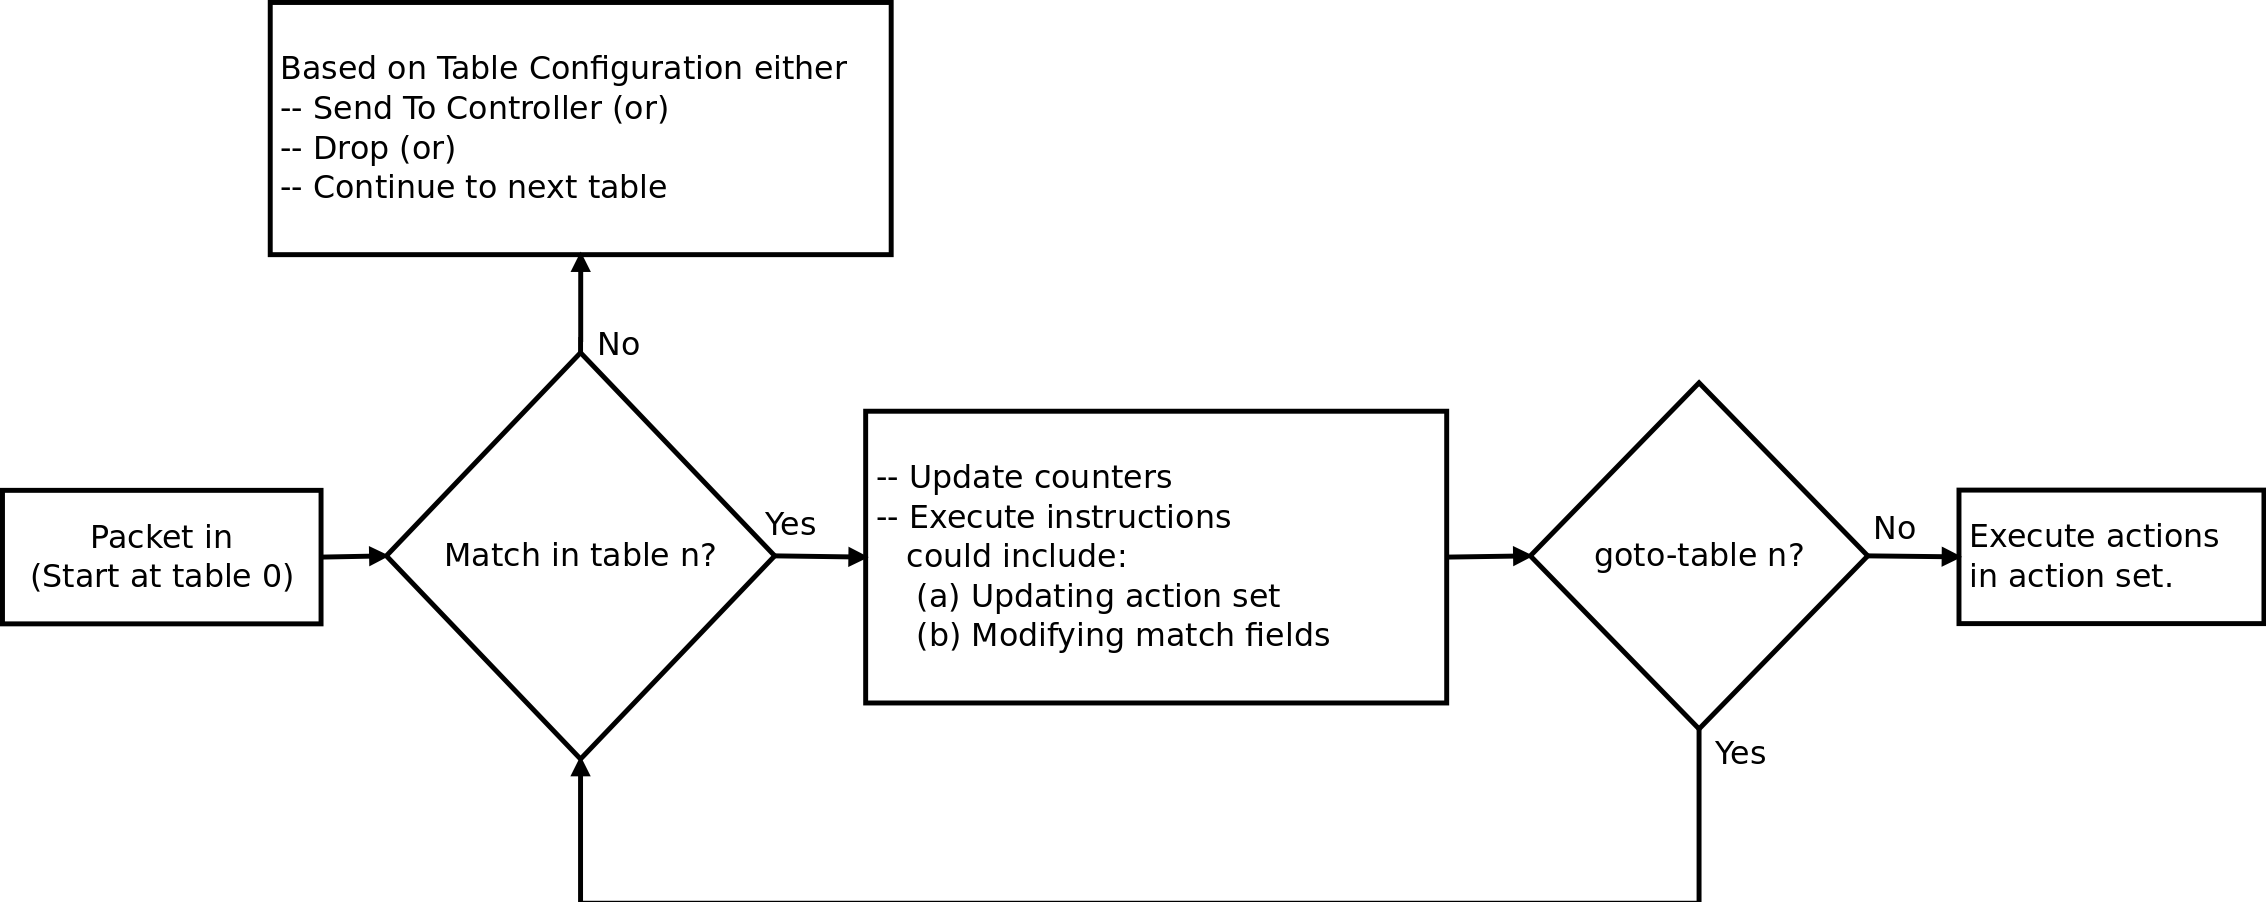
\includegraphics[height=2.0in]{packet_flow_flowchart}
\caption{Flowchart detailing packet flow through an OpenFlow switch.}
\label{fig:packet_flow}
\end{figure}

\begin{figure}[!htb]
\centering
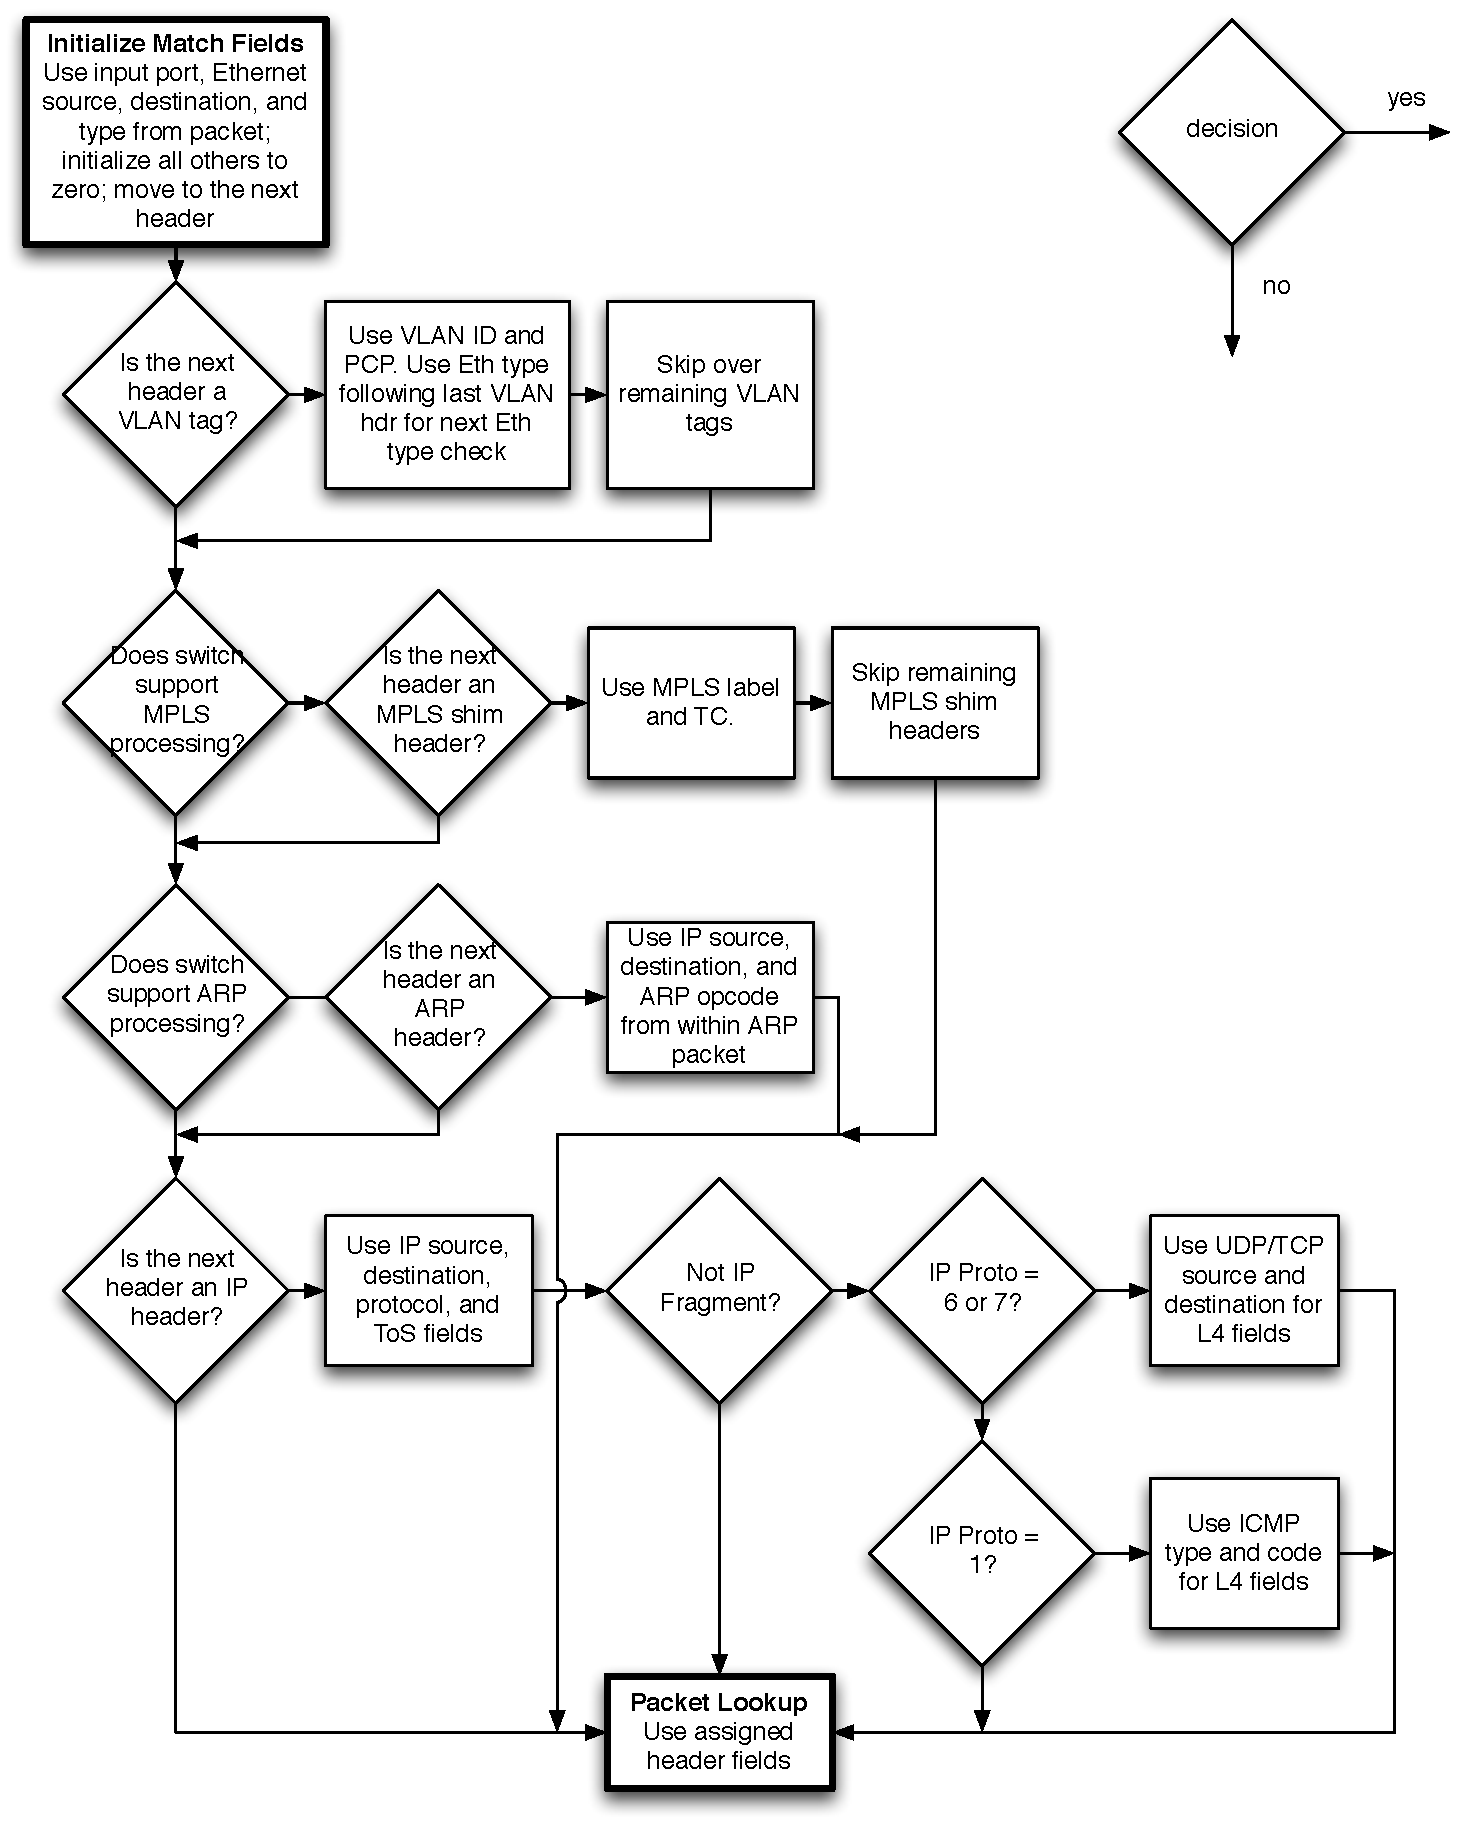
\includegraphics[width=\textwidth]{header_parsing_flowchart}
\caption{Flowchart showing how match fields are parsed for matching.}
\label{fig:header_parsing}
\end{figure}

On receipt of a packet, an OpenFlow Switch performs the functions shown in Figure \ref{fig:packet_flow}. The switch starts by performing a table lookup in the first flow table, and, based on pipeline processing, may perform table lookup in other flow tables (see \ref{sec:pipeline}). Match fields used for table lookups depend on the packet type as in Figure \ref{fig:header_parsing}.
\\\\
A packet matches a flow table entry if the values in the match fields used for the lookup (as defined in Figure~\ref{fig:header_parsing}) match those defined in the flow table.  If a flow table field has a value of ANY, it matches all possible values in the header.  
\\\\
To handle the various Ethernet framing types, matching the Ethernet type is handled in a slightly different manner.  If the packet is an Ethernet II frame, the Ethernet type is handled in the expected way.  If the packet is an 802.3 frame with a SNAP header and Organizationally Unique Identifier (OUI) of 0x000000, the SNAP protocol id is matched against the flow's Ethernet type.  A flow entry that specifies an Ethernet type of 0x05FF, matches all Ethernet 802.2 frames without a SNAP header and those with SNAP headers that do not have an OUI of 0x000000.  
\\\\
The switch should apply the instruction set and update the associated counters of \emph{only} the highest-priority flow entry matching the packet.  If there are multiple matching flow entries with the same highest priority, the matching flow entry is explicitly undefined.  This case can only arise when a controller writer never sets the \verb|CHECK_OVERLAP| bit on flow mod messages and adds overlapping entries.
\\\\
IP fragments must be reassembled before pipeline processing if the switch configuration contains the \verb|OFPC_FRAG_REASM| flag (see~\ref{sec:switch_config}).


\subsection{Counters}

Counters may be maintained for each table, flow, port, queue, group, and bucket.  OpenFlow-compliant counters may be implemented in software and maintained by polling hardware counters with more limited ranges.
\\\\
Table \ref{table:counters} contains the set of counters.  Duration refers to the amount of time the flow has been installed in the switch.  The Receive Errors field is the total of all receive and collision errors defined in Table \ref{table:counters}, as well as any others not called out in the table.  Counters wrap around with no overflow indicator.
\begin{table}[!hbp]
\centering
\footnotesize
%\begin{tabularx}{\textwidth}{ |X|X| }
\begin{tabular}{ |l|c| }
\hline Counter & Bits	 \\
\hline \multicolumn{2}{|c|}{Per Table} \\
\hline Reference count (active entries) & 32 \\
\hline Packet Lookups & 64 \\
\hline Packet Matches & 64 \\
\hline \multicolumn{2}{|c|}{Per Flow} \\
\hline Received Packets & 64 \\
\hline Received Bytes & 64 \\
\hline Duration (seconds) & 32 \\
\hline Duration (nanoseconds) & 32 \\
\hline  \multicolumn{2}{|c|}{Per Port} \\
\hline Received Packets & 64 \\
\hline Transmitted Packets & 64 \\
\hline Received Bytes & 64 \\
\hline Transmitted Bytes & 64 \\
\hline Receive Drops & 64 \\
\hline Transmit Drops & 64 \\
\hline Receive Errors & 64 \\
\hline Transmit Errors & 64 \\
\hline Receive Frame Alignment Errors & 64 \\
\hline Receive Overrun Errors & 64 \\
\hline Receive CRC Errors & 64 \\
\hline Collisions & 64 \\
\hline  \multicolumn{2}{|c|}{Per Queue} \\
\hline Transmit Packets & 64 \\
\hline Transmit Bytes & 64 \\
\hline Transmit Overrun Errors & 64\\
\hline \multicolumn{2}{|c|}{Per Group} \\
\hline Reference Count (flow entries) & 32 \\
\hline Packet Count & 64 \\
\hline Byte Count & 64 \\
\hline \multicolumn{2}{|c|}{Per Bucket} \\
\hline Packet Count & 64 \\
\hline Byte Count & 64 \\
\hline
\end{tabular}
\caption{List of counters}
\label{table:counters}
\end{table}

\subsection{Instructions}
\label{ft:instructions}
Each flow entry contains a set of instructions that are executed when a packet matches the entry. These instructions result in changes to the packet, action set and/or pipeline processing (see: \ref{ft:actionset}). Supported instructions include:
\begin{itemize} 
\item \textbf{Clear-Actions}: Clears all the actions in the action set immediately.
\item \textbf{Apply-Actions \textit{action(s)}}: Applies the specific action(s) immediately, without any change to the Action Set. This instruction may be used to modify the packet between two tables or to execute multiple actions of the same type. The actions are specified as an action list (see \ref{ft:actionlist}).
\item \textbf{Write-Actions \textit{action(s)}}: Merges the specified action(s) into the current action set (see \ref{ft:actionset}).  If an action of the given type exists in the current set, overwrite it, otherwise add it.
\item \textbf{Write-Metadata \textit{metadata / mask}}: Writes the masked metadata value into the metadata field. The mask specifies which bits of the metadata register should be modified (i.e. new\_metadata = old\_metadata \& \~{}mask $|$ value \& mask).
\item \textbf{Goto-Table \textit{next-table-id}}: Indicates the next table in the processing pipeline. The table-id must be greater than the current table-id. The flows of last table of the pipeline can not include this instruction (see \ref{sec:pipeline}).
\end{itemize} 

An instruction set contains a maximum of one instruction of each type. The instructions of the set execute in the order specified by this above list.  In practice, the only constraint is that the Clear-Actions instruction is executed before the Write-Actions instruction.
\\\\
A switch may reject a flow entry if it is unable to execute the instructions associated with the flow entry. In this case, the switch must return an unsupported flow error.  Flow tables may not support every match and every instruction.
\\\\
The instruction set associated with a flow entry contains a maximum of one instruction of each type. The order in which instructions are executed usually does not matter; the exception is that \emph{Clear-Actions} needs to be executed before \emph{Write-Actions}.

\subsection{Action Set}
\label{ft:actionset}
An action set is associated with each packet. This set is empty by default. A flow entry can modify the action set using a \textit{Write-Action} instruction or a \textit{Clear-Action} instruction associated with a particular match. The action set is carried between flow tables. When an instruction set does not contain a \textit{Goto-Table} instruction, pipeline processing stops and the actions in the action set are executed.
\\\\
An action set contains a maximum of one action of each type. When multiple actions of the same type are required, e.g. pushing multiple MPLS labels or popping multiple MPLS labels, the \emph{Apply-Actions} instruction may be used (see \ref{ft:instructions}). The actions of the \emph{Apply-Actions} instruction are executed while executing the instruction, and therefore prior to the execution of the action set.
\\\\
The actions in an action set are applied in the order specified below, regardless of the order that they were added to the set. If an action set contains a group action, the actions in the appropriate action bucket of the group are also applied in the order specified below. The switch may support arbitrary action execution order through the action list of the \textit{Apply-Actions} instruction.

\begin{enumerate}
\item \textbf{copy TTL inwards}: apply copy TTL inward actions to the packet
\item \textbf{pop}: apply all tag pop actions to the packet
\item \textbf{push}: apply all tag push actions to the packet
\item \textbf{copy TTL outwards}: apply copy TTL outwards action to the packet
\item \textbf{decrement TTL}: apply decrement TTL action to the packet
\item \textbf{set}: apply all set-field actions to the packet
\item \textbf{qos}: apply all QoS actions, such as set\_queue to the packet
\item \textbf{group}: if a group action is specified, apply the actions of the relevant group bucket(s) in the order specified by this list
\item \textbf{output}: if no group action is specified, forward the packet on the port specified by the output action
\end{enumerate}

The output action in the action set is executed last. If both an output action and a group action are specified in an action set, the output action is ignored and the group action takes precedence. If no output action and no group action were specified in an action set, the packet is dropped. The execution of groups is recursive; a group bucket may specify another group, in which case the execution of actions traverses all the groups specified by the group configuration.

\subsection{Action List}
\label{ft:actionlist}

The \textit{Apply-Actions} instruction and the \textit{Packet-out} message include an action list. The semantic of the action list is identical to the OpenFlow 1.0 specification. The actions of an action list are executed in the order specified by the list, and are applied immediately to the packet.
\\\\
The execution of action start with the first action in the list and each action is executed on the packet in sequence. The effect of those actions is cumulative, if the action list contains two Push VLAN actions, two VLAN headers are added to the packet. If the action list list contains an output action, a copy of the packet is forwarded in its current state to the desired port. If the list contains a group actions, a copy of the packet in its current state is processed by the relevant group buckets.
\\\\
After the execution of the action list in a \textit{Apply-Actions} instruction, pipeline execution continues, the packet may be matched by subsequent tables as needed and the packet instruction set is executed as needed. The instruction set is unchanged by the execution of the action list.

\subsection{Actions}
\label{ft:actions}
A switch is not required to support all action types --- just those marked ``Required Actions'' below. When connecting to the controller, a switch indicates which of the ``Optional Actions'' it supports.
\\\\
\textbf{Required Action:} \textit{Output}.
The Output action forwards a packet to a specified port. OpenFlow switches must support forwarding to physical ports and switch-defined virtual ports. Standard ports are defined as physical ports, switch-defined virtual ports, and the \verb|LOCAL| port if supported (excluding other reserved virtual ports). OpenFlow switches must also support forwarding to the following reserved virtual ports:
\begin{itemize}
\item \textbf{ALL:} Send the packet out all standard ports, but not to the ingress port or ports that are configured \verb|OFPPC_NO_FWD|.
\item \textbf{CONTROLLER:} Encapsulate and send the packet to the controller.
\item \textbf{TABLE:} Submit the packet to the first flow table so that the packet can be processed through the regular OpenFlow pipeline.  Only valid in the action set of a packet-out message.
\item \textbf{IN\_PORT:} Send the packet out the ingress port. 
\end{itemize}
\textbf{Optional Action:} \textit{Output}.
The switch may optionally support forwarding to the following reserved virtual ports:
\begin{itemize}
\item \textbf{LOCAL:} Send the packet to the switch's local networking stack. The local port enables remote entities to interact with the switch via the OpenFlow network, rather than via a separate control network. With a suitable set of default rules it can be used to implement an in-band controller connection.
\item \textbf{NORMAL:} Process the packet using the traditional non-OpenFlow pipeline of the switch (see \ref{sec:pipeline}). If the switch cannot forward packets from the OpenFlow pipeline to the normal pipeline, it must indicate that it does not support this action.
\item \textbf{FLOOD:} Flood the packet using the normal pipeline of the switch (see \ref{sec:pipeline}). In general, send the packet out all standard ports, but not to the ingress port, or ports that are in \verb|OFPPS_BLOCKED| state. The switch may also use the packet VLAN ID to select which ports to flood to.

\end{itemize}

\emph{OpenFlow-only} switches do not support output actions to the \textbf{NORMAL} port and \textbf{FLOOD} port, while \emph{OpenFlow-hybrid} switches may support them. Forwarding packets to the \textbf{FLOOD} port depends on the switch implementation and configuration, while forwarding using a \textbf{group} of type \textit{all} enables the controller to more flexibly implement flooding (see \ref{sec:group types}).
\\\\
\textbf{Optional Action:} \emph{Set-Queue}. The set-queue action sets the queue id for a packet. When the packet is forwarded to a port using the output action, the queue id determines which queue attached to this port is used for forwarding the packet. Forwarding behavior is dictated by the configuration of the queue and is used to provide basic Quality-of-Service (QoS) support (see section \ref{cts:qos}).
\\\\
\textbf{Required Action:} \emph{Drop}.  There is no explicit action to represent drops.  Instead, packets whose action sets have no output actions should be dropped.  This result could come from empty instruction sets or empty action buckets in the processing pipeline, or after executing a Clear-Actions instruction.
\\\\
\textbf{Optional Action:} \emph{Push-Tag/Pop-Tag}.  Switches may support the ability to push/pop tags as shown in Table \ref{table:push pop actions}.  To aid integration with existing networks, we suggest that the ability to push/pop VLAN tags be supported.

The ordering of header fields/tags is:
\begin{center}
\begin{tabular}{|l|l|l|l|l|}
\hline
Ethernet & VLAN & MPLS & ARP/IP & TCP/UDP/SCTP (IP-only) \\
\hline
\end{tabular}
\end{center}
Newly pushed tags should \emph{always} be inserted as the outermost tag in this ordering. When a new VLAN tag is pushed, it should be the outermost VLAN tag inserted immediately after the Ethernet header. Likewise, when a new MPLS tag is pushed, it should be the outermost MPLS tag, inserted as a shim header after any VLAN tags.
\\\\
Note: Refer to section~\ref{sec:push field defaults} for information on default field values.
\\\\
\textbf{Optional Action:} \emph{Set-Field}.  The various Set-Field actions modify the values of the respective header field in the packet. While not strictly required, the actions shown in Table \ref{table:set-field actions}  greatly increase the usefulness of an OpenFlow implementation.  To aid integration with existing networks, we suggest that VLAN modification actions be supported. Set-Field actions should \emph{always} be applied to the outermost-possible header (e.g.~a ``Set VLAN ID'' action always sets the ID of the outermost VLAN tag).
\\\\
\textbf{Required Action:} \emph{Group}.  Process the packet through the specified group.  The exact interpretation depends on group type. 

\begin{table}[hbp]
\centering
\footnotesize
\begin{tabularx}{\textwidth}{ |l|c|X| }
\hline
Action & Associated Data & Description \\
\hline
Push VLAN header &
Ethertype &
Push a new VLAN header onto the packet.

The Ethertype is used as the Ethertype for the tag. Only Ethertype 0x8100 and 0x88a8 should be used.
\\
\hline
Pop VLAN header &
- &
Pop the outer-most VLAN header from the packet. \\
\hline
Push MPLS header &
Ethertype &
Push a new MPLS shim header onto the packet.

The Ethertype is used as the Ethertype for the header only if the new tag being pushed is the bottom of stack. Only Ethertype 0x8847 and 0x8848 should be used.
\\
\hline
Pop MPLS header &
Ethertype &
Pop the outer-most MPLS tag or shim header from the packet.

The Ethertype is only used when popping the bottom of stack and indicates the Ethertype of the payload.
\\
\hline
\end{tabularx}
\caption{Push/pop tag actions.}
\label{table:push pop actions}
\end{table}

\bottomcaption{Set-Field actions.}
\label{table:set-field actions}
\tablefirsthead{\hline \textbf{Action} & \textbf{Associated Data} &
                       \textbf{Description} \\
		       \hline }
\tablehead{\multicolumn{3}{c}%
           {{\bfseries \tablename\ \thetable{} -- continued from previous page}} \\
           \hline \textbf{Action} & \textbf{Associated Data} &
                  \textbf{Description} \\
	          \hline }
\tablelasthead{\multicolumn{3}{c}%
           {{\bfseries \tablename\ \thetable{} -- concluded from previous page}} \\
           \hline \textbf{Action} & \textbf{Associated Data} &
                  \textbf{Description} \\
	          }
\tabletail{\hline \multicolumn{3}{|r|}{{Continued on next page}} \\ \hline}
\tablelasttail{\hline}
\xentrystretch{0}
\begin{xtabular}{ |p{\atactionwidth}|p{\atassocwidth}|p{\atdescwidth}| }
Set Ethernet source MAC address &
48 bits: New source MAC address &
Replace the existing Ethernet source MAC address. \\
\hline
Set Ethernet destination MAC address &
48 bits: New destination MAC address &
Replace the existing Ethernet destination MAC address. \\
\hline
Set VLAN ID &
12 bits: New VLAN ID &
Replace the existing VLAN ID.
Only applies to packets with an existing VLAN tag. \\
\hline
Set VLAN priority &
3 bits: New VLAN priority &
Replace the existing VLAN priority.
Only applies to packets with an existing VLAN tag. \\
\hline
Set MPLS label &
20 bits: New MPLS label &
Replace the existing MPLS label.
Only applies to packets with an existing MPLS shim header. \\
\hline
Set MPLS traffic class &
3 bits: New MPLS traffic class &
Replace the existing MPLS traffic class.
Only applies to packets with an existing MPLS shim header. \\
\hline
Set MPLS TTL &
8 bits: New MPLS TTL &
Replace the existing MPLS TTL.
Only applies to packets with an existing MPLS shim header. \\
\hline
Decrement MPLS TTL &
- &
Decrement the MPLS TTL.
Only applies to packets with an existing MPLS shim header. \\
\hline
Set IPv4 source address &
32 bits: New IPv4 source address &
Replace the existing IP source address with new value and update the IP checksum (and TCP/UDP/SCTP 
checksum if applicable). 

This action is only applicable to IPv4 packets. \\
\hline
Set IPv4 destination address &
32 bits: New IPv4 destination address &
Replace the existing IP destination address with and update the IP checksum (and TCP/UDP/SCTP checksum if applicable).

This action is only applied to IPv4 packets. \\
\hline
Set IPv4 ToS bits &
6 bits: New IPv4 ToS &
Replace the existing IP ToS and update the IP checksum.
Only applies to IPv4 packets. \\
\hline
Set IPv4 ECN bits &
2 bits: New IPv4 ECN &
Replace the existing IP ECN value and update the IP checksum.
Only applies to IPv4 packets. \\
\hline
Set IPv4 TTL &
8 bits: New IPv4 TTL &
Replace the existing IP TTL and update the IP checksum.
Only applies to IPv4 packets. \\
\hline
Decrement IPv4 TTL &
- &
Decrement the IP TTL field and update the IP checksum.
Only applies to IPv4 packets. \\
\hline
Set transport source port &
16 bits: New TCP, UDP or SCTP source port &
Replace the existing TCP/UDP/SCTP source port with new value and update the TCP/UDP/SCTP checksum.

This action is only applicable to TCP, UDP and SCTP packets.\\
\hline
Set transport destination port &
16 bits: New TCP, UDP or SCTP destination port &
Replace the existing TCP/UDP/SCTP destination port with new value and update the TCP/UDP/SCTP checksum

Only applies to TCP, UDP and SCTP packets.\\
\hline
Copy TTL outwards&
- &
Copy the TTL from next-to-outermost to outermost header with TTL.

Copy can be IP-to-IP, MPLS-to-MPLS, or IP-to-MPLS.
\\
\hline
Copy TTL inwards&
- &
Copy the TTL from outermost to next-to-outermost header with TTL.

Copy can be IP-to-IP, MPLS-to-MPLS, or MPLS-to-IP.
\\
\end{xtabular}

\subsubsection{Default values for fields on push}
\label{sec:push field defaults}
Field values should be copied from existing outer headers to new outer headers when executing a push action. New fields without corresponding existing fields should be set to \emph{zero}. Table~\ref{table:push field copy} details the existing fields from which a new field may take it's value.

\begin{table}[hbp]
\centering
\begin{tabular}{lcl}
\textbf{New Fields} & & \textbf{Existing Field(s)} \\
\hline
VLAN ID & $\leftarrow$ & VLAN ID \\
VLAN priority & $\leftarrow$ & VLAN priority \\
MPLS label & $\leftarrow$ & MPLS label \\
MPLS traffic class & $\leftarrow$ & MPLS traffic class \\
MPLS TTL & $\leftarrow$ &
$\left\{
\begin{array}{l}
  \mathrm{MPLS\ TTL} \\ \mathrm{IP\ TTL}
\end{array}
\right.$ \\
\end{tabular}
\caption{Existing fields that may be copied into new fields on a push action.}
\label{table:push field copy}
\end{table}

Fields in new headers may be overridden by specifying a ``set'' action for the appropriate field(s) after the push operation.

\section{OpenFlow Channel}
The OpenFlow channel is the interface that connects each OpenFlow switch to a controller.  Through this interface, the controller configures and manages the switch, receives events from the switch, and sends packets out the switch.
\\\\
Between the datapath and the OpenFlow channel, the interface is implementation-specific, however all OpenFlow channel messages must be formatted according to the OpenFlow protocol. The OpenFlow channel is usually encrypted using TLS, but may be run directly over TCP.
\\\\
Support for multiple simultaneous controllers is currently undefined.

\subsection{OpenFlow Protocol Overview}
The OpenFlow protocol supports three message types, \emph{controller-to-switch}, \emph{asynchronous}, and \emph{symmetric}, each with multiple sub-types.  Controller-to-switch messages are initiated by the controller and used to directly manage or inspect the state of the switch.  Asynchronous messages are initiated by the switch and used to update the controller of network events and changes to the switch state. Symmetric messages are initiated by either the switch or the controller and sent without solicitation.  The message types used by OpenFlow are described below.

\subsubsection{Controller-to-Switch}
Controller/switch messages are initiated by the controller and may or may not require a response from the switch.
\\\\
\textbf{Features}:  The controller may request the capabilities of a switch by sending a features request; the switch must respond with a features reply that specifies the capabilities of the switch. This is commonly performed upon establishment of the OpenFlow channel.
\\\\
\textbf{Configuration}: The controller is able to set and query configuration parameters in the switch.  The switch only responds to a query from the controller.
\\\\
\textbf{Modify-State}: Modify-State messages are sent by the controller to manage state on the switches.  Their primary purpose is to add/delete and modify flows/groups in the OpenFlow tables and to set switch port properties.
\\\\
\textbf{Read-State}: Read-State messages are used by the controller to collect statistics from the switch.
\\\\
\textbf{Packet-out}:  These are used by the controller to send packets out of a specified port on the switch, and to forward packets received via Packet-in messages. Packet-out messages must contain a full packet or a buffer ID referencing a packet stored in the switch. The message must also contain a list of actions to be applied in the order they are specified; an empty action list drops the packet.
\\\\
\textbf{Barrier}: Barrier request/reply messages are used by the controller to ensure message dependencies have been met or to receive notifications for completed operations.  

\subsubsection{Asynchronous}
\label{sec:asynchronous}
Asynchronous messages are sent without the controller soliciting them from a switch.  Switches send asynchronous messages to the controller to denote a packet arrival, switch state change, or error.  The four main asynchronous message types are described below.
\\\\
\textbf{Packet-in:} For all packets that do not have a matching flow entry, a packet-in event may be sent to the controller (depending on the table configuration). For all packets forwarded to the \textbf{CONTROLLER} virtual port, a packet-in event is always sent to the controller.  If the switch has sufficient memory to buffer packets that are sent to the controller, the packet-in events contain some fraction of the packet header (by default \input{define/OFP_DEFAULT_MISS_SEND_LEN} bytes) and a buffer ID to be used by the controller when it is ready for the switch to forward the packet.  Switches that do not support internal buffering (or have run out of internal buffering) must send the full packet to the controller as part of the event. Buffered packets will usually be processed via a \textbf{Packet-out} message from the controller, or automatically expired after some time.
\\\\
\textbf{Flow-Removed:} When a flow entry is added to the switch by a flow modify message, an idle timeout value indicates when the entry should be removed due to a lack of activity, as well as a hard timeout value that indicates when the entry should be removed, regardless of activity.  The flow modify message also specifies whether the switch should send a flow removed message to the controller when the flow expires.  Flow delete requests should generate flow removed messages for any flows with the \verb|OFPFF_SEND_FLOW_REM| flag set.
\\\\
\textbf{Port-status:} The switch is expected to send port-status messages to the controller as port configuration state changes.  These events include change in port status events (for example, if it was brought down directly by a user).
\\\\
\textbf{Error:} The switch is able to notify the controller of problems using error messages. 

\subsubsection{Symmetric}
Symmetric messages are sent without solicitation, in either direction.
\\\\
\textbf{Hello:} Hello messages are exchanged between the switch and controller upon connection startup.
\\\\
\textbf{Echo:} Echo request/reply messages can be sent from either the switch or the controller, and must return an echo reply.  They can be used to measure the latency or bandwidth of a controller-switch connection, as well as verify its liveness.
\\\\
\textbf{Experimenter:} Experimenter messages provide a standard way for OpenFlow switches to offer additional functionality within the OpenFlow message type space.  This is a staging area for features meant for future OpenFlow revisions.

\subsection{Connection Setup}
The switch must be able to establish communication with a controller at a user-configurable (but otherwise fixed) IP address, using a user-specified port.  If the switch knows the IP address of the controller, the switch initiates a standard TLS or TCP connection to the controller.  Traffic to and from the OpenFlow channel is not run through the OpenFlow pipeline.  Therefore, the switch must identify incoming traffic as local before checking it against the flow tables.  Future versions of the protocol specification will describe a dynamic controller discovery protocol in which the IP address and port for communicating with the controller is determined at runtime.
\\\\
When an OpenFlow connection is first established, each side of the connection must immediately send an \verb|OFPT_HELLO| message with the \verb|version| field set to the highest OpenFlow protocol version supported by the sender.  Upon receipt of this message, the recipient may calculate the OpenFlow protocol version to be used as the smaller of the version number that it sent and the one that it received.
\\\\
If the negotiated version is supported by the recipient, then the connection proceeds. Otherwise, the recipient must reply with an \verb|OFPT_ERROR| message with a \verb|type| field of \verb|OFPET_HELLO_FAILED|, a \verb|code| field of \verb| OFPHFC_COMPATIBLE|, and optionally an ASCII string explaining the situation in \verb|data|, and then terminate the connection.

\subsection{Connection Interruption}
In the case that a switch loses contact with the current controller, as a result of an echo request timeout, TLS session timeout, or other disconnection, it should attempt to contact one or more backup controllers.  The ordering by which a switch contacts backup controllers is not specified by the protocol.
\\\\
The switch should \emph{immediately} enter either ``fail secure mode'' or ``fail standalone mode'' if it loses connection to the controller, depending upon the switch implementation and configuration. In ``fail secure mode'', the only change to switch behavior is that packets and messages destined to the current controller are dropped. Flows should continue to expire according to their timeouts in ``fail secure mode''. In ``fail standalone mode'', the switch processes all packets using the \verb|OFPP_NORMAL| port; in other words, the switch acts as a legacy Ethernet switch or router.
\\\\
Upon connecting to a controller again, the existing flow entries remain.  The controller then has the option of deleting all flow entries, if desired.
\\\\
The first time a switch starts up, it will operate in either ``fail secure mode'' or ``fail standalone mode'' mode.  Configuration of the default set of flow entries to be used at startup is outside the scope of the OpenFlow protocol.

\subsection{Encryption}
The switch and controller may communicate through a TLS connection.  The TLS connection is initiated by the switch on startup to the controller, which is located by default on TCP port \input{define/OFP_TCP_PORT}.   The switch and controller mutually authenticate by exchanging certificates signed by a site-specific private key.  Each switch must be user-configurable with one certificate for authenticating the controller (controller certificate) and the other for authenticating to the controller (switch certificate).

\subsection{Flow Table Modification Messages}
\label{sec:flow mod messages}
\label{flow_table:sec_chan:flow_add}
\label{flow_table:sec_chan:flow_mod}
\label{flow_table:sec_chan:flow_removal}
Flow table modification messages can have the following types:
\input{enum/ofp_flow_mod_command}
For ADD requests with the \verb|OFPFF_CHECK_OVERLAP| flag set, the switch must first check for any overlapping flow entries.  Two flow entries overlap if a single packet may match both, and both entries have the same priority.  If an overlap conflict exists between an existing flow entry and the ADD request, the switch must refuse the addition and respond with an \verb|ofp_error_msg| with \verb|OFPET_FLOW_MOD_FAILED| type and \verb|OFPFMFC_OVERLAP| code.
\\\\
For valid (non-overlapping) ADD requests, or those with no overlap checking, the switch must insert the flow entry to the requested table.  If a flow entry with identical match fields and priority already resides in the requested table, then that entry, including its counters and duration, must be cleared from the table, and the new flow entry added. No flow-removed message is generated for the flow entry eliminated as part of an ADD request ; if the controller wants a flow-removed message it should explicitly send a DELETE\_STRICT for the old flow prior to adding the new one.

\\\\
For MODIFY requests, if a flow entry with identical match fields does not current reside in any table, the MODIFY acts like an ADD, and the new flow entry must be inserted with zeroed counters.  If a matching entry exist in the table, the timeout fields and actions field of this entry are changed the the new values, whereas its counters and duraction fields are left unchanged.
\\\\
For DELETE requests, if no flow entry matches, no error is recorded, and no flow table modification occurs.  If flow entries match, and must be deleted, then each entry with the \verb|OFPFF_SEND_FLOW_REM| flag set should generate a flow removed message.
\\\\
MODIFY and DELETE flow mod commands have corresponding \_STRICT versions.   Without \_STRICT appended, the wildcards are active and all flows that match the description are modified or removed.  If \_STRICT is appended, all fields, including the wildcards and priority, are strictly matched against the entry, and only an identical flow is modified or removed.  For example, if a message to remove entries is sent that has all the wildcard flags set, the DELETE command would delete all flows from all tables, while the DELETE\_STRICT command would only delete a rule that applies to all packets at the specified priority.
\\\\
For non-strict MODIFY and DELETE commands that contain wildcards, a match will occur when a flow entry exactly matches or is more specific than the description in the flow\_mod command. For example, if a DELETE command says to delete all flows with a destination port of 80, then a flow entry that is all wildcards will not be deleted. However, a DELETE command that is all wildcards will delete an entry that matches all port 80 traffic.  This same interpretation of mixed wildcard and exact match fields also applies to individual and aggregate flows stats.  
\\\\
DELETE and DELETE\_STRICT commands can be optionally filtered by destination group or output port.  If the \verb|out_port| field contains a value other than \verb|OFPP_ANY|, it introduces a constraint when matching.  This constraint is that each matching rule must contain a \emph{set-output-port} action directed at the specified port in the actions associated with that rule.  This constraint is limited to only the actions directly associated with the rule.  In other words, the switch must not recurse through the action sets of pointed-to groups, which may have matching \emph{set-output-port} actions.  The \verb|out_group|, if different from \verb|OFPG_ANY|, introduce a similar constraint on the \emph{group} action. These fields are ignored by ADD, MODIFY, and MODIFY\_STRICT messages.
\\\\
MODIFY, MODIFY\_STRICT, DELETE and DELETE\_STRICT commands can also be filtered by cookie value, if the \verb|cookie_mask| field contains a value other than 0. This constraint is that the bits specified by the \verb|cookie_mask| in both the \verb|cookie| field of the flow mod and a flow's \verb|cookie| value must be equal. In other words, (flow.cookie \& flow\_mod.cookie\_mask) == (flow\_mod.cookie \& flow\_mod.cookie\_mask).

\\\\
If the flow modification message specifies an invalid table, the switch should send an \verb|ofp_error_msg| with \verb|OFPET_FLOW_MOD_FAILED| type and \verb|OFPFMFC_BAD_TABLE_ID| code.
\\\\
If a switch cannot find any space in the requested table in which to add the incoming flow entry, the switch should send an \verb|ofp_error_msg| with \verb|OFPET_FLOW_MOD_FAILED| type and \verb|OFPFMFC_TABLE_FULL| code.
\\\\
If the match fields requested in a flow mod message are unsupported in the table, the switch must return an \verb|ofp_error_msg| with \verb|OFPET_FLOW_MOD_FAILED| type and \verb|OFPFMC_BAD_MATCH| code.
\\\\
If the instructions requested in a flow mod message are unsupported, the switch must return an \verb|ofp_error_msg| with \verb|OFPET_FLOW_MOD_FAILED| type and \verb|OFPFMC_BAD_INSTRUCTION| code.
\\\\
If the match in a flow mod specifies an arbitrary bitmask for either the datalink or network addresses which the switch cannot support, the switch must return an \verb|ofp_error_msg| with \verb|OFPET_FLOW_MOD_FAILED| type and either \verb|OFPFMFC_BAD_DL_ADDR_MASK| or \verb|OFPFMFC_BAD_NW_ADDR_MASK|. (If the bitmasks specified in \emph{both} the datalink and network addresses are not supported then \verb|OFPFMFC_BAD_DL_ADDR_MASK| should be used.)
\\\\
In the match in a flow mod specifies values that can not be matched, for example a VLAN ID greater than 4095 and not one of the reserved value, or a ToS value with one of the two lower bit set, the switch may return an \verb|ofp_error_msg| with \verb|OFPET_FLOW_MOD_FAILED| type and \verb|OFPFMFC_BAD_MATCH| code.
\\\\
If any action references a port that will never be valid on a switch, the switch must return an \verb|ofp_error_msg| with \verb|OFPET_BAD_ACTION| type and \verb|OFPBAC_BAD_OUT_PORT| code.  If the referenced port may be valid in the future, e.g. when a linecard is added to a chassis switch, or a port is dynamically added to a software switch, the switch may either silently drop packets sent to the referenced port, or immediately return an \verb|OFPBAC_BAD_OUT_PORT| error and refuse the flow mod.
\\\\
If an action in a flow mod message references a group that is not currently defined on the switch, or is a reserved group, such as \verb|OFPG_ALL|, the switch must return an \verb|ofp_error_msg| with \verb|OFPET_BAD_ACTION| type and \verb|OFPBAC_BAD_OUT_GROUP| code.
\\\\
If an action in a flow mod message has a value that is invalid, for example a Set VLAN ID action with value greater than 4095, or a Push action with an invalid Ethertype, the switch should return an \verb|ofp_error_msg| with \verb|OFPET_BAD_ACTION| type and \verb|OFPBAC_BAD_ARGUMENT| code.
\\\\
If an action in a flow mod message performs an operation which is inconsistent with the match, for example, a pop VLAN action with a match specifying no VLAN, or a set IPv4 address action with a match wildcarding the Ethertype, the switch must apply this action conditionally to only packets where it can be performed (in the above example, IPv4 packet would have their IPv4 address rewritten and non-IPv4 packets would be left unchanged). If the switch can not implement this behaviour, it must reject the flow and must immediately return an \verb|ofp_error_msg| with \verb|OFPET_BAD_ACTION| type and \verb|OFPBAC_MATCH_INCONSISTENT| code.
\\\\
If any other errors occur during the processing of the flow mod message, the switch may return an  \verb|ofp_error_msg| with \verb|OFPET_FLOW_MOD_FAILED| type and \verb|OFPFMC_UNKNOWN| code.
\subsection{Flow Removal}

Each flow entry has an \verb|idle_timeout| and a \verb|hard_timeout| associated with it.  If no packet has matched the rule in the last \verb|idle_timeout| seconds, or it has been \verb|hard_timeout| seconds since the flow was inserted, the switch removes the entry and sends a flow removed message.  In addition, the controller is able to actively remove entries by sending a flow message with the \verb|DELETE| or \verb|DELETE_STRICT| command.  Like the message used to add the entry, a removal message contains a description, which may include wild cards.

\subsection{Group Table Modification Messages}
\label{group_table:sec_chan:group_mod}
\label{group_table:sec_chan:group_add}
\label{group_table:sec_chan:group_set}
\label{group_table:sec_chan:group_delete}
Group table modification messages can have the following types:
\input{enum/ofp_group_mod_command}

The action set for each bucket must be validated using the same rules as those for flow mods (Section \ref{flow_table:sec_chan:flow_add}), with additional group-specific checks. If an action in one of the buckets is invalid or unsupported, the switch should return an \verb|ofp_error_msg| with \verb|OFPET_BAD_ACTION| type and code corresponding to the error (see \ref{flow_table:sec_chan:flow_add}).
\\\\
Groups may consist of zero or more buckets. A group with no buckets will not alter the action set associated with a packet. A group may also include buckets which themselves forward to other groups. For example, a fast reroute group may have two buckets, where each points to a select group. If a switch does not support groups of groups, it must send an \verb|ofp_error_msg| with \verb|OFPET_GROUP_MOD_FAILED| type and \verb|OFPGMFC_CHAINING_UNSUPPORTED| code.  If a group mod is sent such that a forwarding loop would be created, the switch should send an \verb|ofp_error_msg| with \verb|OFPET_GROUP_MOD_FAILED| type and \verb|OFPGMFC_LOOP| code.  If the switch does not support such checking, the forwarding behavior is undefined.
\\\\
For ADD requests, if a group entry with the specified group identifier already resides in the group table, then the switch must refuse to add the group entry and must send an \verb|ofp_error_msg| with \verb|OFPET_GROUP_MOD_FAILED| type and \verb|OFPGMFC_GROUP_EXISTS| code.
\\\\
For MODIFY requests, if a group entry with the specified group identifier already resides in the group table, then that entry, including its type and action buckets, must be removed, and the new group entry added. If a group entry with the specified group identifier does not already exist then the switch must refuse the group mod and send an \verb|ofp_error_msg| with \verb|OFPET_GROUP_MOD_FAILED| type and \verb|OFPGMFC_UNKNOWN_GROUP| code.
\\\\
If a specified group type is invalid (ie: includes fields such as \verb|weight| that are undefined for the specified group type) then the switch must refuse to add the group entry and must send an \verb|ofp_error_msg| with \verb|OFPET_GROUP_MOD_FAILED| type and \verb|OFPGMFC_INVALID_GROUP| code.
\\\\
If a switch does not support unequal load sharing with select groups (buckets with weight different than 1), it must refuse to add the group entry and must send an \verb|ofp_error_msg| with \verb|OFPET_GROUP_MOD_FAILED| type and \verb|OFPGMFC_WEIGHT_UNSUPPORTED| code.
\\\\
If a switch cannot add the incoming group entry due to lack of space, the switch must send an \verb|ofp_error_msg| with \verb|OFPET_GROUP_MOD_FAILED| type and \verb|OFPGMFC_OUT_OF_GROUPS| code.
\\\\
If a switch cannot add the incoming group entry due to restrictions (hardware or otherwise) limiting the number of group buckets, it must refuse to add the group entry and must send an \verb|ofp_error_msg| with \verb|OFPET_GROUP_MOD_FAILED| type and \verb|OFPGMFC_OUT_OF_BUCKETS| code.
\\\\
If a switch cannot add the incoming group because it does not support the proposed liveliness configuration, the switch must send an \verb|ofp_error_msg| with \verb|OFPET_GROUP_MOD_FAILED| type and \verb|OFPGMFC_WATCH_UNSUPPORTED| code. This includes specifying \verb|watch_port| or \verb|watch_group| for a group that does not support liveness, or specifying a port that does not support liveness in \verb|watch_port|, or specifying a group that does not support liveness in \verb|watch_group|.
\\\\
For DELETE requests, if no group entry with the specified group identifier currently exists in the group table, no error is recorded, and no group table modification occurs.  Otherwise, the group is removed, and all flows that forward to the group are also removed. The group type need not be specified for the DELETE request. DELETE also differs from an ADD or MODIFY with no buckets specified in that future attempts to ADD the group identifier will not result in a group exists error.  If one wishes to effectively delete a group yet leave in flow entries using it, that group can be cleared by sending a MODIFY with no buckets specified.
\\\\
To delete all groups with a single message, specify \verb|OFPG_ALL| as the group value.
\\\\
Fast failover group support requires liveness monitoring, to determine the specific bucket to execute. Other group types are not required to implement liveness monitoring, but may optionally implement it.  If a switch cannot implement liveness checking for any bucket in a group, it must refuse the group mod and return an error.  The rules for determining liveness include:
\begin{itemize}
\item A port is considered live if it has the \verb|OFPPS_LIVE| flag set in its port state.  Port liveness may be managed by code outside of the OpenFlow portion of a switch, defined outside of the OpenFlow spec (such as Spanning Tree or a KeepAlive mechanism).  At a minimum, the port should not be considered live if the port config bit \verb|OFPPC_PORT_DOWN| indicates the port is down, or if the port state bit \verb|OFPPS_LINK_DOWN| indicates the link is down.
\item A bucket is considered live if either \verb|watch_port| is not \verb|OFPP_ANY| and the port watched is live, or if \verb|watch_group| is not \verb|OFPG_ANY| and the group watched is live.
\item A group is considered live if a least one of its buckets is live.
\end{itemize}

The controller can infer the liveness state of the group by monitoring the states of the various ports.

\appendixtitleon
\begin{appendices}
%\appendix
\section{Appendix A: The OpenFlow Protocol}
The heart of the OpenFlow spec is the set of structures used for OpenFlow Protocol messages.  
\\\\
The structures, defines, and enumerations described below are derived from the file \verb|include/openflow/openflow.h|, which is part of the standard OpenFlow distribution.  All structures are packed with padding and 8-byte aligned, as checked by the assertion statements.  All OpenFlow messages are sent in big-endian format.  

\subsection{OpenFlow Header}
Each OpenFlow message begins with the OpenFlow header:

\input{struct/ofp_header}
The version specifies the OpenFlow protocol version being used.  During the current draft phase of the OpenFlow Protocol, the most significant bit will be set to indicate an experimental version and the lower bits will indicate a revision number.  The current version is \input{define/OFP_VERSION}.  The final version for a Type 0 switch will be 0x00.  The length field indicates the total length of the message, so no additional framing is used to distinguish one frame from the next.  The type can have the following values:

\input{enum/ofp_type}

\subsection{Common Structures}
This section describes structures used by multiple messages.

\subsubsection{Port Structures}
Ports are described with the following structure:

\input{struct/ofp_port}
The \verb|port_no| field is a value the datapath associates with a port. The \verb|hw_addr| field typically is the MAC address for the port; \verb|OFP_MAX_ETH_ALEN| is 6.  The name field is a null-terminated string containing a human-readable name for the interface.  The value of \verb|OFP_MAX_PORT_NAME_LEN| is 16.  
\\\\
The \verb|config| field describes administrative settings with the following structure:

\input{enum/ofp_port_config}
The port config bits indicate whether a port has been administratively brought down and how to handle incoming and outgoing packets.
\\\\
When the port flags are changed, the switch sends an \verb|OFPT_PORT_STATUS| message to notify the controller of the change. The \verb|OFPPFL_NO_RECV|, \verb|OFPPFL_NO_FWD|, and \verb|OFPPFL_NO_PACKET_IN| bits in the OpenFlow port flags may be useful for the controller to implement protocols such as STP or BFD.
\\\\
The \verb|state| field describes the physical link state with the following structure:

\input{enum/ofp_port_state}
All port state bits are read-only, representing the state of the physical link or switch protocols outside of OpenFlow. The \verb|OFPPS_LINK_DOWN| bit indicates the the physical link is not present. The \verb|OFPPS_BLOCKED| bit indicates that a switch protocol outside of OpenFlow, such as 802.1D Spanning Tree, is preventing the use of that port with \verb|OFPP_FLOOD|.
\\\\
The port numbers use the following conventions:

\input{enum/ofp_port_no}
The \verb|curr|, \verb|advertised|, \verb|supported|, and \verb|peer| fields indicate link modes (speed and duplexity), link type (copper/fiber) and link features (autonegotiation and pause).  Port features are represented by the following structure:

\input{enum/ofp_port_features}
Multiple of these flags may be set simultaneously. If none of the port speed flags are set, the \verb|max_speed| or \verb|curr_speed| are used.
\\\\
The \verb|curr_speed| and \verb|max_speed| fields indicate the current and maximum bit rate (raw transmission speed) of the link in kbps. The number should be rounded to match common usage. For example, an optical 10 Gb Ethernet port should have this field set to 10000000 (instead of 10312500), and an OC-192 port should have this field set to 10000000 (instead of 9953280).

\subsubsection{\qosupd{Queue Structures}}
\label{cts:qos}
\qosupd{An OpenFlow switch provides limited Quality-of-Service support
  (QoS) through a simple queuing
mechanism. One (or more) queues can attach to a port and be used to map flows
on it. Flows mapped to a specific queue will be treated according to
that queue's configuration (e.g. min rate).
\\\\
A queue is described by the} \verb|ofp_packet_queue| \qosupd{structure:
\input{struct/ofp_packet_queue}
Each queue is further described by a set of properties, each of a
specific type and configuration.
\input{enum/ofp_queue_properties}
Each queue property description starts with a common header:
\input{struct/ofp_queue_prop_header}
Currently, there is only a minimum-rate type queue, described by the}
\verb|ofp_queue_prop_min_rate| \qosupd{structure:
\input{struct/ofp_queue_prop_min_rate}}

\subsubsection{Flow Match Structures}
When describing a flow entry, the following structure is used:

\input{struct/ofp_match}
The \verb|wildcards| field has a number of flags that may be set:

\input{enum/ofp_flow_wildcards}

The metadata field is used to pass information between lookups across multiple tables. This value can be masked using the metadata mask (which is 0xFFFFFFFFFFFFFFFF by default). If the metadata wildcard bit is set, the contents of these fields are ignored in the lookup.
\\\\
There are also four match field masks: \verb|dl_src_mask|, \verb|dl_dst_mask|, \verb|nw_src_mask|, and \verb|nw_dst_mask|. These mask fields allow the corresponding fields (\verb|dl_src|, \verb|dl_dst|, \verb|nw_src|, and \verb|nw_dst|) to be masked arbitrarily. The masks are defined such that a 1 in a given bit position indicates a ``don't care'' match for the same bit in the corresponding field, whereas a 0 means match the bit exactly.
\\\\
If no wildcards are set and the \verb|_mask| fields are all zero, then the \verb|ofp_match| exactly describes a flow, over the entire OpenFlow n-tuple.  On the other extreme, if all the wildcard flags and \verb|_mask| fields are set, then every flow will match.
\\\\
Setting the \verb|OFPFW_DL_VLAN| or \verb|OFPFW_MPLS_LABEL| bits specifies that flow should match packets regardless of whether they contain the corresponding tag. Special values are defined for the VLAN tag and MPLS label to allow the matching of packets without a tag, or packets with a tag independent of the tag's value. The special values defined for \verb|dl_vlan| are:
\input{enum/ofp_vlan_id}
The special values defined for \verb|mpls_label| are:
\input{enum/ofp_mpls_label}
Tables~\ref{table:vlan wildcards} and \ref{table:mpls wildcards} summarize the combinations of wildcard bits and field values for particular matches.

\begin{table}[hbp]
\centering
\begin{tabularx}{\textwidth}{|c|c|X|}
\hline
Wildcard bit & \verb|dl_vlan| value & Matching packets \\
\hline
\verb|OFPFW_DL_VLAN| & * & Packets with and without a VLAN tag \\
\hline
- & \verb|OFPVID_NONE| & Only packets \emph{without} a VLAN tag \\
\hline
- & \verb|OFPVID_ANY| & Only packets \emph{with} a VLAN tag regardless of it's value \\
\hline
\end{tabularx}
\caption{Match combinations for VLAN tags.}
\label{table:vlan wildcards}
\end{table}

\begin{table}[hbp]
\centering
\begin{tabularx}{\textwidth}{|c|c|X|}
\hline
Wildcard bit & \verb|mpls_label| value & Matching packets \\
\hline
\verb|OFPFW_MPLS_LABEL| & * & Packets with and without a MPLS shim header \\
\hline
- & \verb|OFPML_NONE| & Only packets \emph{without} a MPLS shim header \\
\hline
- & \verb|OFPML_ANY| & Only packets \emph{with} a MPLS shim header regardless of it's value \\
\hline
\end{tabularx}
\caption{Match combinations for MPLS headers.}
\label{table:mpls wildcards}
\end{table}

\subsubsection{Flow Instruction Structures}
Flow instructions associated with a flow table entry are executed when a flow matches the entry. The list of instructions that are currently defined are:

\input{enum/ofp_instruction_type}
The instruction set is described in section \ref{ft:instructions}.  Flow tables may support a subset of instruction types.

\input{struct/ofp_instruction_goto_table}
\verb|table_id| indicates the next table in the packet processing pipeline.

\input{struct/ofp_instruction_write_metadata}
Metadata for the next table lookup can be written using the \verb|metadata| and the \verb|metadata_mask| in order to set specific bits on the match field.   If this instruction is not specified, the metadata is passed, unchanged.

\input{struct/ofp_instruction_actions}
This structure is used for all actions related instructions. For the Clear-Actions instruction, the structure does not contain any actions.

\subsubsection{Action Structures}
A number of actions may be associated with flows, groups or packets.  The currently defined action types are:

\input{enum/ofp_action_type} 
Output, group, \qosupd{and set-queue} actions are described in Section~\ref{ft:actions}, tag push/pop actions are described in Table~\ref{table:push pop actions}, and Field-Modify actions are described in Table~\ref{table:field modify actions}.  An action definition contains the action type, length, and any associated data:

\input{struct/ofp_action_header}
An \verb|action_output| has the following fields:

\input{struct/ofp_action_output}
The \verb|max_len| indicates the maximum amount of data from a packet that should be sent when the port is \verb|OFPP_CONTROLLER|.  If \verb|max_len| is zero, the switch must send a zero-size \verb|packet_in| message.  The \verb|port| specifies the port through which the packet should be sent.
\\\\
An \verb|action_group| has the following fields:

\input{struct/ofp_action_group}
The \verb|group_id| indicates the group used top process this packet.  The set of buckets to apply depends on the group type.
\\\\
\qosupd{The set-queue action sets the queue id that will be used to map a flow to an already-configured queue, regardless of the TOS and VLAN PCP bits.
  The packet should not change after an set-queue action. If the switch
  needs to set the TOS/PCP bits for internal handling, the original values
  should be restored before sending the packet out.
\\\\
A switch may support only queues that are tied to specific PCP/TOS
bits. In that case, we cannot map an arbitrary flow to a specific
queue, therefore the action SET-QUEUE is not supported. The user can
still use these queues and map
flows to them by setting the relevant fields (TOS, VLAN PCP).
\\\\
An } \verb|action_set_queue| \qosupd{has the following fields:

\input{struct/ofp_action_set_queue}}
An \verb|action_vlan_vid| has the following fields:

\input{struct/ofp_action_vlan_vid}
The \verb|vlan_vid| field is 16 bits long, when an actual VLAN id is only 12 bits. The value \verb|0xffff| is used to indicate that no VLAN id was set.
\\\\
An \verb|action_vlan_pcp| has the following fields:

\input{struct/ofp_action_vlan_pcp}
The \verb|vlan_pcp| field is 8 bits long, but only the lower 3 bits have meaning.  
\\\\
An \verb|action_mpls_label| has the following fields:

\input{struct/ofp_action_mpls_label}
The \verb|mpls_label| field is 32 bits long, but only the lower 20 bits have meaning.
\\\\
An \verb|action_mpls_tc| has the following fields:

\input{struct/ofp_action_mpls_tc}
The \verb|mpls_tc| field is 8 bits long, but only the lower 3 bits have meaning.
\\\\
An \verb|action_mpls_ttl| has the following fields:

\input{struct/ofp_action_mpls_ttl}
The \verb|mpls_ttl| field is the MPLS TTL to set.
\\\\
An \verb|action_dec_mpls_ttl| takes no arguments and consists only of a generic \verb|ofp_action_header|. The action decrements the MPLS TTL.
\\\\
An \verb|action_dl_addr| has the following fields:

\input{struct/ofp_action_dl_addr}
The \verb|dl_addr| field is the MAC address to set.
\\\\
An \verb|action_nw_addr| has the following fields:

\input{struct/ofp_action_nw_addr}
The \verb|nw_addr| field is the IP address to set.
\\\\
An \verb|action_nw_tos| has the following fields:

\input{struct/ofp_action_nw_tos}
The \verb|nw_tos| field is the 6 upper bits of the ToS field to set, in the original bit positions (shifted to the left by 2).
\\\\
An \verb|action_nw_ttl| has the following fields:

\input{struct/ofp_action_nw_ttl}
The \verb|nw_ttl| field is the TTL address to set in the IP header.
\\\\
An \verb|action_dec_nw_ttl| takes no arguments and consists only of a generic \verb|ofp_action_header|.  This action decrement the TTL in the IP header if one is present.
\\\\
An \verb|action_tp_port| has the following fields:

\input{struct/ofp_action_tp_port}
The \verb|tp_port| field is the TCP/UDP/other port to set.
\\\\
An \verb|action_copy_ttl_out| takes no arguments and consists only of a generic \verb|ofp_action_header|. The action copies the TTL from the next-to-outermost header with TTL to the outermost header with TTL.
\\\\
An \verb|action_copy_ttl_in| takes no arguments and consists only of a generic \verb|ofp_action_header|. The action copies the TTL from the outermost header with TTL to the next-to-outermost header with TTL.
\\\\
An \verb|action_push| has the following fields:

\input{struct/ofp_action_push}
The \verb|ethertype| indicates the Ethertype of the new tag. It is used when pushing any new VLAN tags and the bottom of stack MPLS header.
\\\\
An \verb|action_pop_vlan| takes no arguments and consists only of a generic \verb|ofp_action_header|. The action pops the outermost VLAN tag from the packet.
\\\\
An \verb|action_pop_mpls| has the following fields:

\input{struct/ofp_action_pop_mpls}
The \verb|ethertype| indicates the Ethertype of the payload and is only used when popping the bottom of stack.
\\\\
An \verb|action_experimenter| has the following fields:

\input{struct/ofp_action_experimenter_header}
The \verb|experimenter| field is the Experimenter ID, which takes the same form as in struct \verb|ofp_experimenter|.

\subsection{Controller-to-Switch Messages}

\subsubsection{Handshake}
\label{cts:handshake} 
Upon TLS session establishment, the controller sends an \verb|OFPT_FEATURES_REQUEST| message.  This message does not contain a body beyond the OpenFlow header.  The switch responds with an \verb|OFPT_FEATURES_REPLY| message:

\input{struct/ofp_switch_features}
The \verb|datapath_id| field uniquely identifies a datapath.  The lower 48 bits are intended for the switch MAC address, while the top 16 bits are up to the implementer.  An example use of the top 16 bits would be a VLAN ID to distinguish multiple virtual switch instances on a single physical switch.  This field should be treated as an opaque bit string by controllers.
\\\\
The \verb|n_tables| field describes the number of tables supported by the switch, each of which can have a different set of supported wildcard bits and number of entries.  When the controller and switch first communicate, the controller will find out how many tables the switch supports from the Features Reply. If it wishes to understand the size, types, and order in which tables are consulted, the controller sends a \verb|OFPST_TABLE| stats request. A switch must return these tables in the order the packets traverse the tables, with all exact-match tables listed before all tables with wildcards.
\\\\
The \verb|capabilities| field uses the following flags:

\input{enum/ofp_capabilities} 
The \verb|actions| field is a bitmap of actions supported by the switch.  The list of actions is found in Section~\ref{ft:actions}; all actions marked Required must be supported. Experimenter actions should \emph{not} be reported via this bitmask. The bitmask uses the values from \verb|ofp_action_type| as the number of bits to shift left for an associated action. For example, \verb|OFPAT_SET_DL_VLAN| would use the flag \verb|0x00000002|.
\\\\
The \verb|ports| field is an array of \verb|ofp_port| structures that describe all the ports in the system that support OpenFlow.  The number of port elements is inferred from the length field in the OpenFlow header. 

\subsubsection{Switch Configuration}
The controller is able to set and query configuration parameters in the switch with the \verb|OFPT_SET_CONFIG| and \verb|OFPT_GET_CONFIG_REQUEST| messages, respectively.  The switch responds to a configuration request with an \verb|OFPT_GET_CONFIG_REPLY| message; it does not reply to a request to set the configuration.  
\\\\
There is no body for \verb|OFPT_GET_CONFIG_REQUEST| beyond the OpenFlow header.  The \verb|OFPT_SET_CONFIG| and \verb|OFPT_GET_CONFIG_REPLY| use the following:

\input{struct/ofp_switch_config}
The configuration flags include the following:

\input{enum/ofp_config_flags}
The \verb|OFPC_FRAG_*| flags indicate whether IP fragments should be treated normally, dropped, or reassembled.  ``Normal" handling of fragments means that an attempt should be made to pass the fragments through the OpenFlow tables. If any field is not present (e.g., the TCP/UDP ports didn't fit), then the packet should not match any entry that has that field set.
\\\\
The \verb|OFPC_INVALID_TTL_TO_CONTROLLER| flag indicates whether packets with invalid IP TTL or MPLS TTL should be dropped or sent to the controller.  The flag is cleared by default, causing invalid packets to get dropped.
\\\\
The \verb|miss_send_len| field defines the number of bytes of each packet sent to the controller as a result of both flow table misses and flow table hits with the controller as the destination.  If this field equals 0, the switch must send a zero-size \verb|packet_in| message.

\subsubsection{Flow Table Configuration}
The controller can configure and query table state in the switch with the \verb|OFP_TABLE_MOD| and \verb|OFPST_TABLE_STATS| requests, respectively. The switch responds to a table stats request with a \verb|OFPT_STATS_REPLY| message.

\input{struct/ofp_table_mod}
The \verb|table_id| chooses the table to which the configuration change should be applied. If the \verb|table_id| is \verb|0xFF|, the configuration is applied to all tables in the switch.

The \verb|config| field is a bitmap that is used to configure the default behavior of unmatched packets.  By default, any packet that does not match a table is sent to the controller for processing using a \verb|OFPT_PACKET_IN| message.  This behavior can be modified by using the following flags:

\input{enum/ofp_table_config}
The \verb|OFPTC_TABLE_MISS_CONTINUE| flag directs unmatched packets to the next table in the pipeline, except for the last table of the pipeline where unmatched packets are sent to the controller.  This behavior is similar to the multiple table match process in the OpenFlow 1.0 specification. The \verb|OFPTC_TABLE_MISS_DROP| flag drops unmatched packets.

\subsubsection{Modify State Messages}
\paragraph{Modify Flow Entry Message}
Modifications to the flow table from the controller are done with the \verb|OFPT_FLOW_MOD| message:

\input{struct/ofp_flow_mod}
The \verb|cookie| field is an opaque data value that is set by the
controller.  It is not used in any packet-matching functions, and thus does
not need to reside in hardware.  The value -1 (0xffffffffffffffff) is
reserved and must not be used.  It is required that when \verb|command| is
\verb|OFPC_MODIFY| or \verb|OFPC_MODIFY_STRICT| that matched flows have
their \verb|cookie| field updated with the new value.
\\\\
The \verb|cookie_mask| field's behavior is explained in Section \ref{flow_table:sec_chan:flow_add}. It is used only to filter flows, then discarded.
\\\\
The \verb|table_id| field specifies the table into which the flow should be inserted.
Table 0 signifies the first table in the pipeline.
\\\\
The \verb|command| field must be one of the following:

\input{enum/ofp_flow_mod_command}
The differences between \verb|OFPFC_MODIFY| and \verb|OFPFC_MODIFY_STRICT| are explained in Section \ref{flow_table:sec_chan:flow_mod} and differences between \verb|OFPFC_DELETE| and \verb|OFPFC_DELETE_STRICT| are explained in Section \ref{flow_table:sec_chan:flow_removal}. 
\\\\
The \verb|idle_timeout| and \verb|hard_timeout| fields control how quickly flows expire.  
\\\\
If the \verb|idle_timeout| is set and the \verb|hard_timeout| is zero, the entry must expire after \verb|idle_timeout| seconds with no received traffic.  If the \verb|idle_timeout| is zero and the \verb|hard_timeout| is set, the entry must expire in \verb|hard_timeout| seconds regardless of whether or not packets are hitting the entry.
\\\\
If both \verb|idle_timeout| and \verb|hard_timeout| are set, the flow will timeout after \verb|idle_timeout| seconds with no traffic, or \verb|hard_timeout| seconds, whichever comes first.  If both \verb|idle_timeout| and \verb|hard_timeout| are zero, the entry is considered permanent and will never time out.  It can still be removed with a \verb|flow_mod| message of type \verb|OFPFC_DELETE|. 
\\\\
The \verb|priority| indicates priority within the specified flow table table. Higher numbers indicate higher priorities.
\\\\
The \verb|buffer_id| refers to a buffered packet sent by the \verb|OFPT_PACKET_IN| message.
\\\\
The \verb|out_port| and \verb|out_group| fields optionally filter the scope of DELETE and DELETE\_STRICT messages by output port and group.  If either \verb|out_port| or \verb|out_group| contains a value other than \verb|OFPP_NONE| or \verb|OFPG_NONE| respectively, it introduces a constraint when matching.  This constraint is that the rule must contain an output action directed at that port or group.  Other constraints such as \verb|ofp_match| structs and priorities are still used; this is purely an \emph{additional} constraint.  Note that to disable output filtering, both \verb|out_port| and \verb|out_group| must be set to \verb|OFPP_NONE| and \verb|OFPG_NONE| respectively.  This field is ignored by ADD, MODIFY, and MODIFY\_STRICT messages.
\\\\
The \verb|flags| field may include the follow flags:

\input{enum/ofp_flow_mod_flags}
When the \verb|OFPFF_SEND_FLOW_REM| flag is set, the switch must send a flow removed message when the flow expires.  The default is for the switch to not send flow removed messages for newly added flows.  
\\\\
When the \verb|OFPFF_CHECK_OVERLAP| flag is set, the switch must check that there are no conflicting entries with the same priority. If there is one, the flow mod fails and an error code is returned.

\paragraph{Modify Group Entry Message}
Modifications to the group table from the controller are done with the \verb|OFPT_GROUP_MOD| message:

\input{struct/ofp_group_mod}
The semantics of the type and group fields are explained in \ref{group_table:sec_chan:group_mod}.
\\\\
The \verb|command| field must be one of the following:

\input{enum/ofp_group_mod_command}
The \verb|type| field must be one of the following:

\input{enum/ofp_group_type}
Buckets use the following struct:

\input{struct/ofp_bucket}
The \verb|weight| field is only defined for multipath groups.  The bucket's share of the traffic processed by the group is defined by the individual bucket's weight divided by the sum of the bucket weights in the group.  When a port goes down, the change in traffic distribution is undefined.  The precision by which a switch's packet distribution should match bucket weights is undefined.
\\\\
The \verb|watch_port| and \verb|watch_group| fields are only required for fast failover groups, and may be optionally implemented for other group types.  These fields indicate the port and/or group whose liveness controls whether this bucket is a candidate for forwarding.  For fast failover groups, the first bucket defined is the highest-priority bucket, and only the highest-priority live bucket is used.

\paragraph{Port Modification Message}
The controller uses the \verb|OFPT_PORT_MOD| message to modify the behavior of the port:

\input{struct/ofp_port_mod}
The \verb|mask| field is used to select bits in the \verb|config| field to change.  The \verb|advertise| field has no mask; all port features change together.

\subsubsection{\qosupd{Queue Configuration Messages}}
\qosupd{Queue configuration takes place outside the OpenFlow protocol, either
  through a command line tool or through an external dedicated configuration
protocol.
\\\\
The controller can query the switch for configured queues on a port
using the following structure:
\input{struct/ofp_queue_get_config_request}
The switch replies back with an} \verb|ofp_queue_get_config_reply| \qosupd{command, containing
a list of configured queues.

\input{struct/ofp_queue_get_config_reply}
}

\subsubsection{Read State Messages}
While the system is running, the datapath may be queried about its current state using the \verb|OFPT_STATS_REQUEST| message:

\input{struct/ofp_stats_request}
The switch responds with one or more \verb|OFPT_STATS_REPLY| messages:

\input{struct/ofp_stats_reply}
The only value defined for \verb|flags| in a reply is whether more replies will follow this one - this has the value \verb|0x0001|.  To ease implementation, the switch is allowed to send replies with no additional entries.  However, it must always send another reply following a message with the �more� flag set.  The transaction ids (xid) of replies must always match the request that prompted them.
\\\\
In both the request and response, the \verb|type| field specifies the kind of information being passed and determines how the \verb|body| field is interpreted:

\input{enum/ofp_stats_types}

\paragraph{Description Statistics}
Information about the switch manufacturer, hardware revision, software revision, serial number, and a description field is available from the \verb|OFPST_DESC| stats request type:

\input{struct/ofp_desc_stats}
Each entry is ASCII formatted and padded on the right with null bytes (\textbackslash0).  \verb|DESC_STR_LEN| is \input{define/DESC_STR_LEN}and \verb|SERIAL_NUM_LEN| is \input{define/SERIAL_NUM_LEN}.  Note: \footnote{Added to address concerns raised in \url{https://mailman.stanford.edu/pipermail/openflow-spec/2009-September/000504.html}} the \verb|dp_desc| field is a free-form string to describe the datapath for debugging purposes, e.g., ``switch3 in room 3120''.  As such, it is not guaranteed to be unique and should not be used as the primary identifier for the datapath---use the \verb|datapath_id| field from the switch features instead (\S~\ref{cts:handshake}).

\paragraph{Individual Flow Statistics}
Information about individual flows is requested with the \verb|OFPST_FLOW| stats request type:

\input{struct/ofp_flow_stats_request}
The \verb|match| field contains a description of the flows that should be matched and may contain wildcards.  This field's matching behavior is described in Section \ref{flow_table:sec_chan:flow_add}.
\\\\
The \verb|table_id| field indicates the index of a single table to read, or \verb|0xff| for all tables.
\\\\
The \verb|out_port| field optionally filters by output port.  If \verb|out_port| contains a value other than \verb|OFPP_NONE|, it introduces a constraint when matching.  This constraint is that the rule must contain an output action directed at that port.  Other constraints such as \verb|ofp_match| structs are still used; this is purely an \emph{additional} constraint.  Note that to disable output port filtering, \verb|out_port| must be set to \verb|OFPP_NONE|. 
\\\\
The usage of the \verb|cookie| and \verb|cookie_mask| fields is defined in Section \ref{flow_table:sec_chan:flow_add}.
\\\
The \verb|body| of the reply consists of an array of the following:

\input{struct/ofp_flow_stats}
The fields consist of those provided in the \verb|flow_mod| that created these, plus the table into which the entry was inserted, the packet count, and the byte count.
\\\\
\label{flow_duration_info}The \verb|duration_sec| and \verb|duration_nsec| fields indicate the elapsed time the flow has been installed in the switch. The total duration in nanoseconds can be computed as $\verb|duration_sec|*10^{9}$ + \verb|duration_nsec|. Implementations are required to provide millisecond precision; higher precision is encouraged where available.

\paragraph{Aggregate Flow Statistics}
Aggregate information about multiple flows is requested with the \verb|OFPST_AGGREGATE| stats request type:

\input{struct/ofp_aggregate_stats_request}

The fields in this message have the same meanings as in the individual flow stats request type (\verb|OFPST_FLOW|).
\\\\
The \verb|body| of the reply consists of the following:

\input{struct/ofp_aggregate_stats_reply} 

\paragraph{Table Statistics}
Information about tables is requested with the \verb|OFPST_TABLE| stats request type.  The request does not contain any data in the body.
\\\\
The body of the reply consists of an array of the following:

\input{struct/ofp_table_stats}
The \verb|body| contains a \verb|wildcards| field, which indicates the fields for which that particular table supports wildcarding. For example, a direct look-up hash table would have that field set to zero, while a sequentially searched table would have it set to \verb|OFPFW_ALL|. The entries are returned in the order that packets traverse the tables. 
\\\\
The \verb|actions| field is a bitmap of actions supported by the table.  The list of actions is found in Section~\ref{ft:actions}. Experimenter actions should \emph{not} be reported via this bitmask. The bitmask uses the values from \verb|ofp_action_type| as the number of bits to shift left for an associated action. For example, \verb|OFPAT_SET_DL_VLAN| would use the flag \verb|0x00000002|.
\\\\
\verb|OFP_MAX_TABLE_NAME_LEN| is \input{define/OFP_MAX_TABLE_NAME_LEN}.

\paragraph{Port Statistics}
Information about ports is requested with the \verb|OFPST_PORT| stats request type:

\input{struct/ofp_port_stats_request}
The \verb|port_no| field optionally filters the stats request to the given port.  To request all port statistics, \verb|port_no| must be set to \verb|OFPP_NONE|.
\\\\
The \verb|body| of the reply consists of an array of the following:

\input{struct/ofp_port_stats}
The switch should return a value of -1 for unavailable counters.

\paragraph{\qosupd{Queue Statistics}}
\qosupd{The} \verb|OFPST_QUEUE| \qosupd{stats request message provides
  queue statistics for one or more ports.
  The request body consists of a} \verb|port_no| \qosupd{field
identifying the port and a} \verb|queue_id|. \verb|OFPP_ALL|
\qosupd{refers to all ports, while} \verb|OFPQ_ALL| \qosupd{refers to all queues configured
at a port.

\input{struct/ofp_queue_stats_request}
The body of the reply consists of an array of
the following structure:

\input{struct/ofp_queue_stats}}
\paragraph{Group Statistics}
The \verb|OFPST_GROUP| stats request message provides statistics for one or more groups.  The request body consists of a \verb|group_id| field, which can be set to \verb|OFPG_ALL| to refer to all groups on the switch.

\input{struct/ofp_group_stats_request}
The body of the reply consists of an array of the following structure:

\input{struct/ofp_group_stats}
The \verb|bucket_stats| field consists of an array of \verb|ofp_bucket_counter| structs:

\input{struct/ofp_bucket_counter}
The switch should return a value of -1 for unavailable counters.
\paragraph{Group Description Statistics}
The \verb|OFPST_GROUP_DESC| stats request message provides a way to list the set of groups on a switch, along with their corresponding bucket actions.  The request body is empty, while the reply body is an array of the following structure:

\input{struct/ofp_group_desc_stats}
Fields for group description stats are the same as those used with the \verb|ofp_group_mod| struct.

\paragraph{Experimenter Statistics}
Experimenter-specific stats messages are requested with the \verb|OFPST_EXPERIMENTER| stats type. The first four bytes of the message are the experimenter identifier. The rest of the body is experimenter-defined.
\\\\
The \verb|experimenter| field is a 32-bit value that uniquely identifies the experimenter. If the most significant byte is zero, the next three bytes are the experimenter's IEEE OUI. If experimenter does not have (or wish to use) their OUI, they should contact the OpenFlow consortium to obtain one. 

\subsubsection{Send Packet Message}
When the controller wishes to send a packet out through the datapath, it uses the \verb|OFPT_PACKET_OUT| message:

\input{struct/ofp_packet_out}
The \verb|buffer_id| is the same given in the \verb|ofp_packet_in| message.  If the \verb|buffer_id| is -1, then the packet data is included in the data array. If \verb|OFPP_TABLE| is specified as the output port of an action, the \verb|in_port| in the \verb|packet_out| message is used in the flow table lookup.

\subsubsection{Barrier Message}
When the controller wants to ensure message dependencies have been met or wants to receive notifications for completed operations, it may use an \verb|OFPT_BARRIER_REQUEST| message.  This message has no body.  Upon receipt, the switch must finish processing all previously-received messages before executing any messages beyond the Barrier Request.  When such processing is complete, the switch must send an \verb|OFPT_BARRIER_REPLY| message with the \verb|xid| of the original request.

\subsection{Asynchronous Messages}
\subsubsection{Packet-In Message}
When packets are received by the datapath and sent to the controller, they use the \verb|OFPT_PACKET_IN| message:

\input{struct/ofp_packet_in}
The \verb|in_phy_port| is the physical port on which the packet was received. The \verb|in_port| is the virtual port through which a packet was received, or physical port if the packet was not received on a virtual port.  For example, if a packet is received on a tunnel interface, the \verb|in_port| is the tunnel port\_no and the \verb|in_phy_port| is the physical port\_no on which the tunnel is configured. If a packet is received directly on a physical port and not processed by a virtual port, \verb|in_port| should have the same value as \verb|in_phy_port|.
\\\\
The \verb|buffer_id| is an opaque value used by the datapath to identify a buffered packet.  When a packet is buffered, some number of bytes from the message will be included in the data portion of the message.  If the packet is sent because of a ``send to controller'' action, then \verb|max_len| bytes from the \verb|action_output| of the flow setup request are sent.  If the packet is sent because of a flow table miss, then at least \verb|miss_send_len| bytes from the \verb|OFPT_SET_CONFIG| message are sent.  The default \verb|miss_send_len| is \input{define/OFP_DEFAULT_MISS_SEND_LEN}bytes.  If the packet is not buffered, the entire packet is included in the data portion, and the \verb|buffer_id| is -1.  
\\\\
Switches that implement buffering are expected to expose, through documentation, both the amount of available buffering, and the length of time before buffers may be reused.  A switch must gracefully handle the case where a buffered \verb|packet_in| message yields no response from the controller.  A switch should prevent a buffer from being reused until it has been handled by the controller, or some amount of time (indicated in documentation) has passed.
\\\\
The reason field can be any of these values:

\input{enum/ofp_packet_in_reason}
 
\subsubsection{Flow Removed Message}
If the controller has requested to be notified when flows time out, the datapath does this with the \verb|OFPT_FLOW_REMOVED| message:

\input{struct/ofp_flow_removed}
The \verb|match|, \verb|cookie|, and \verb|priority| fields are the same as those used in the flow setup request.
\\\\
The \verb|reason| field is one of the following:

\input{enum/ofp_flow_removed_reason}
The \verb|duration_sec| and \verb|duration_nsec| fields are described in Section \ref{flow_duration_info}.
\\\\
The \verb|idle_timeout| field is directly copied from the flow mod that created this entry. 
\\\\
With the above three fields, one can find both the amount of time the flow was active, as well as the amount of time the flow received traffic.
\\\\
The \verb|packet_count| and \verb|byte_count| indicate the number of packets and bytes that were associated with this flow, respectively. 
 
\subsubsection{Port Status Message}
As ports are added, modified, and removed from the datapath, the controller needs to be informed with the \verb|OFPT_PORT_STATUS| message:

\input{struct/ofp_port_status}
The \verb|status| can be one of the following values:

\input{enum/ofp_port_reason} 

\subsubsection{Error Message}
There are times that the switch needs to notify the controller of a problem.  This is done with the \verb|OFPT_ERROR_MSG| message: 	

\input{struct/ofp_error_msg}
The \verb|type| value indicates the high-level type of error.  The \verb|code| value is interpreted based on the type.  The \verb|data| is variable length and interpreted based on the \verb|type| and \verb|code|; in most cases this is the message that caused the problem.  
\\\\
Error codes ending in \verb|_EPERM| correspond to a permissions error generated by an entity between a controller and switch, such as an OpenFlow hypervisor. 
\\\\
Currently defined error types are:

\input{enum/ofp_error_type}
For the \verb|OFPET_HELLO_FAILED| error \verb|type|, the following \verb|code|s are currently defined:

\input{enum/ofp_hello_failed_code}
The \verb|data| field contains an ASCII text string that adds detail on why the error occurred.
\\\\
For the \verb|OFPET_BAD_REQUEST| error \verb|type|, the following \verb|code|s are currently defined:

\input{enum/ofp_bad_request_code}
The \verb|data| field contains at least 64 bytes of the failed request.
\\\\
For the \verb|OFPET_BAD_ACTION| error \verb|type|, the following \verb|code|s are currently defined:

\input{enum/ofp_bad_action_code}
The \verb|data| field contains at least 64 bytes of the failed request.
\\\\
For the \verb|OFPET_FLOW_MOD_FAILED| error \verb|type|, the following \verb|code|s are currently defined:

\input{enum/ofp_flow_mod_failed_code}
The \verb|data| field contains at least 64 bytes of the failed request.
\\\\
For the \verb|OFPET_GROUP_MOD_FAILED| error \verb|type|, the following \verb|code|s are currently defined:

\input{enum/ofp_group_mod_failed_code}
The \verb|data| field contains at least 64 bytes of the failed request.
\\\\
For the \verb|OFPET_PORT_MOD_FAILED| error \verb|type|, the following \verb|code|s are currently defined:

\input{enum/ofp_port_mod_failed_code}
The \verb|data| field contains at least 64 bytes of the failed request.
\\\\
For the \verb|OFPET_QUEUE_OP_FAILED| error \verb|type|, the following \verb|code|s are currently defined:

\input{enum/ofp_queue_op_failed_code}
The \verb|data| field contains at least 64 bytes of the failed request.
\\\\
If the error message is in response to a specific message from the controller, e.g., \verb|OFPET_BAD_REQUEST|, \verb|OFPET_BAD_ACTION|, or \verb|OFPET_FLOW_MOD_FAILED|, then the \verb|xid| field of the header should match that of the offending message.

\subsection{Symmetric Messages}
\subsubsection{Hello}
The \verb|OFPT_HELLO| message has no body; that is, it consists only of an OpenFlow header. Implementations must be prepared to receive a hello message that includes a body, ignoring its contents, to allow for later extensions. 

\subsubsection{Echo Request}
An Echo Request message consists of an OpenFlow header plus an arbitrary-length data field.  The data field might be a message timestamp to check latency, various lengths to measure bandwidth, or zero-size to verify liveness between the switch and controller.

\subsubsection{Echo Reply}
An Echo Reply message consists of an OpenFlow header plus the unmodified data field of an echo request message.
\\\\
In an OpenFlow protocol implementation divided into multiple layers, the echo request/reply logic should be implemented in the "deepest" practical layer.  For example, in the OpenFlow reference implementation that includes a userspace process that relays to a kernel module, echo request/reply is implemented in the kernel module.  Receiving a correctly formatted echo reply then shows a greater likelihood of correct end-to-end functionality than if the echo request/reply were implemented in the userspace process, as well as providing more accurate end-to-end latency timing.

\subsubsection{Experimenter}
The Experimenter message is defined as follows:

\input{struct/ofp_experimenter_header}
The \verb|experimenter| field is a 32-bit value that uniquely identifies the experimenter. If the most significant byte is zero, the next three bytes are the experimenter's IEEE OUI. If experimenter does not have (or wish to use) their OUI, they should contact the OpenFlow consortium to obtain one. The rest of the body is uninterpreted.
\\\\
If a switch does not understand a experimenter extension, it must send an \verb|OFPT_ERROR| message with a \verb|OFPBRC_BAD_EXPERIMENTER| error code and \verb|OFPET_BAD_REQUEST| error type. 



\section{Appendix B: Credits}

Current Maintainer: Brandon Heller (brandonh@stanford.edu).
\\\\
Spec contributions, in alphabetical order:
\\\\
Ben Pfaff,
Brandon Heller,
Dan Cohn,
Dan Talayco,
David Erickson,
Edward Crabbe,
Glen Gibb,
Guido Appenzeller,
Jean Tourrilhes,
Justin Pettit,
KK Yap,
Martin Casado,
Masayoshi Kobayashi,
Nick McKeown,
Peter Balland,
Rajiv Ramanathan,
Reid Price,
Rob Sherwood,
Yiannis Yiakoumis.

\end{appendices}
 
\end{document} 
